%==================================================
%               DEV2 - Algorithmique
%                HEB - ESI
%
%                 Syllabus
%--------------------------------------------------
% À compiler avec pdflatex
%                                     Marco Codutti
%==================================================

\documentclass[a4paper,twoside]{style-esi/syllabus}
%\includeonly{syllabus/tableau2D}

%=========================
% Les styles
%=========================
\usepackage{style-esi/licence}
\usepackage{style-esi/links}
\usepackage{style-esi/images}
\usepackage{style-esi/exercice}
\usepackage{style-esi/exemple}
\usepackage{style-esi/listing}
\usepackage{style-esi/algo}

\usepackage{textcomp}	        % Plein de symboles

%---------------------------------------
% Pour mettre une icone en marge
% Utilisation: \marginicon{nomIcone}
% L'icone doit être présente dans le dossier icon
% dans un format reconnu (pas de gif)
%---------------------------------------
\usepackage{marginnote}
\newcommand{\marginicon}[1]{%
	\marginnote{\includegraphics[width=16px]{icon/#1}}[0pt]%
}

\usepackage{environ} % Permet de définir un environnement en 1 partie
\newif\ifprintsolutions
\NewEnviron{Solution}{\ifprintsolutions%
	\subsubsection*{\color{colmain}Solution de l'exercice~\arabic{Exercice}.}
	\BODY
	\fi
}

% ========================================================
%  Permet d'ajouter des graphiques Tikz (flow charts,...)
% ========================================================

% === Pour faire des dessins via TikZ
\usepackage{tikz}
\usetikzlibrary{matrix}
\usetikzlibrary{shapes.geometric,arrows}
\usetikzlibrary{positioning}

% === Synopsis adaptés aux nombres d'entrées et de sorties

\newcommand{\flowalgod}[3]{
	\begin{tikzpicture}
		\sffamily
		\matrix [column sep = 2em] {
		 \node (P1) {#1}; \pgfmatrixnextcell \node[draw, rounded corners, thick] (M) {#2}; \pgfmatrixnextcell \node (R) {#3}; \\
		};
		\draw[->,thick] (P1) to (M);
		\draw[->,thick] (M)  to (R);
	\end{tikzpicture}
}

\newcommand{\flowalgodd}[4]{
	\begin{tikzpicture}
		\sffamily
		\matrix [column sep = 2em] {
		 \node (P1) {#1}; \pgfmatrixnextcell \pgfmatrixnextcell \\
		 \pgfmatrixnextcell \node[draw, rounded corners, thick] (M) {#3}; \pgfmatrixnextcell \node (R) {#4}; \\
		 \node (P2) {#2}; \pgfmatrixnextcell \pgfmatrixnextcell \\		          
		};
		\draw[->,thick] (P1) to (M);
		\draw[->,thick] (P2) to (M);
		\draw[->,thick] (M)  to (R);
	\end{tikzpicture}
}

\newcommand{\flowalgoddd}[5]{
	\begin{tikzpicture}
		\sffamily
		\matrix [column sep = 2em] {
		 \node (P1) {#1}; \pgfmatrixnextcell \pgfmatrixnextcell \\
		 \node (P2) {#2}; \pgfmatrixnextcell \node[draw, rounded corners, thick] (M) {#4}; \pgfmatrixnextcell \node (R) {#5}; \\
		 \node (P3) {#3}; \pgfmatrixnextcell \pgfmatrixnextcell \\		          
		};
		\draw[->,thick] (P1) to (M);
		\draw[->,thick] (P2) to (M);
		\draw[->,thick] (P3) to (M);
		\draw[->,thick] (M)  to (R);
	\end{tikzpicture}
}

\newcommand{\flowalgorrr}[5]{
	\begin{tikzpicture}
		\sffamily
		\matrix [column sep = 2em] {
		                  \pgfmatrixnextcell                                               \pgfmatrixnextcell \node (R1) {#3};  \\
		 \node (D1) {#1}; \pgfmatrixnextcell \node[draw, rounded corners, thick] (M) {#2}; \pgfmatrixnextcell \node (R2) {#4}; \\
		                  \pgfmatrixnextcell                                               \pgfmatrixnextcell \node (R3) {#5}; \\		          
		};
		\draw[->,thick] (D1) to (M);
		\draw[->,thick] (M) to (R1);
		\draw[->,thick] (M) to (R2);
		\draw[->,thick] (M) to (R3);
	\end{tikzpicture}
}

\newcommand{\flowalgov}[2]{
	\begin{tikzpicture}
		\sffamily
		\matrix [column sep = 2em] {
		 \node (V) {#1}; \pgfmatrixnextcell \node[draw, rounded corners, thick] (M) {#2}; \\
		};
		\draw[->,thick] (V) to (M);
		\draw[->,thick] (M) to (V);
	\end{tikzpicture}
}

% ========================================================
% Introduit l'environnement Fiche pour des fiches d'algo
% avec numérotation automatique et
% liste des fiches (via \listoffiche)
%
%	\begin{Fiche}{nom fiche}
%		\Section{nom section}
%			...
%		\Section{nom section}
%			...
%	\end{Fiche}
% ========================================================
\usepackage{tocloft}
\usepackage{fancybox}

\newcounter{fichenum}
\setcounter{fichenum}{0}
\newenvironment{Fiche}[1]{%
	\refstepcounter{fichenum}%
	%\clearpage
	\begin{center}
		\Large\sffamily
		\color{MidnightBlue}
		\Ovalbox{\quad{}Fiche \no \thefichenum\ -- #1\quad\rule[-1mm]{0cm}{6mm}}
	\end{center}
	\addcontentsline{toc}{section}{#1}
	\addcontentsline{fic}{fiche}
	{\protect\numberline{\thefichenum}#1}
	\vspace{5mm}
	}{%
	}
\newcommand{\Section}[1]{\vspace*{-3mm}\subsubsection*{\large{\color{MidnightBlue}\hskip-8mm #1}}\vspace*{-1mm}}
\newcommand{\listfichename}{}
\newlistof{fiche}{fic}{\listfichename}

%\printsolutionstrue

%==============================
% Paramètres du document
%==============================
\title{Algorithmique}
\subtitle{Bachelor en Informatique\\DEV2}
\date{2019}
\author{%
	M. Codutti (MCD), H. Delannoy (HDE),\\
	S. Drobisz (SDR), A. Paquot (APA) \& N. Richard (NRI)
}

%==============================
% Document
%==============================

\begin{document}

	\maketitle
	\pagedeux	
	\ccbysa{esi-dev2-list@he2b.be}
	\setcounter{tocdepth}{1}
	\tableofcontents

	% ====================================
\chapter{Les tableaux à 2 dimensions}
% ====================================

% ===================
\section{Définition}
% ===================

	\marginicon{definition}
	La \textbf{dimension} d’un tableau est le nombre d’indices qu’on utilise
	pour faire référence à un de ses éléments. Attention de ne pas confondre 
	avec la	taille !
	
	En \abbr{dev1}, nous avons introduit les tableaux à une dimension.
	Un seul indice suffisait à localiser un de ses éléments. 
	Pour le dire autrement,
	chaque case possédait \textbf{un} numéro.
	De nombreuses situations nécessitent cependant l’usage de tableaux à deux dimensions.
	Ils vous sont déjà familiers par leur présence dans beaucoup de
	situations courantes : calendrier, grille horaire, grille de mots
	croisés, sudoku, jeux se déroulant sur un quadrillage (damier,
	échiquier, scrabble\dots).
	Dans ces situations, 
	chaque case est désignée par \textbf{deux} numéros.

% ====================
\section{Notations}
% ====================

	\subsection{Déclarer}
	%====================
		
		\marginicon{definition}
		Pour \textbf{déclarer} un tableau à 2 dimensions, on écrira :
	
		\begin{algo}
			\Decl{nomTableau}{\Array{nbLignes $\times$ nbColonnes}{TypeElément}}\;
		\end{algo}
	
		où \lda{nbLignes} et \lda{nbColonnes} 
		sont des expressions entières quelconques.
	
		\textbf{Exemple} :
		
		\begin{algo}
			\Decl{tab}{\Array{5$\times$10}{integers}}\;
		\end{algo}
		
		déclare un tableau de 5 lignes par 10 colonnes dont chaque case
		contient un entier.
		
	\subsection{Utiliser}
	%====================

		\marginicon{definition}
		Pour \textbf{accéder} à une case du tableau on donnera les deux indices
		entre crochets.
		Comme en \abbr{dev1}, on considère que la première ligne 
		et la première colonne portent le numéro (l'indice) $0$.  
		
		\textbf{Exemple} :
		
		\begin{algo}
			\Write tab[2,4]
				\RComment{affiche le 5\ieme{} élément de la 3\ieme{} ligne du tableau nommé \samp{tab}.}
		\end{algo}
		
	\subsection{Visualiser}
	%======================

		Notez que la vue sous forme de tableau avec des lignes
		et des colonnes est une vision humaine.
		Il n'y a pas de lignes ni de colonnes en mémoire.
		Pour être précis,
		on devrait juste parler de première dimension et
		de deuxième dimension
		mais la notion de ligne et de colonne
		est un abus de langage qui simplifie le discours.
		
		On pourrait aussi visualiser un tableau à deux dimensions
		comme un tableau à une dimension dont chacun des éléments est
		lui-même un tableau à une dimension.
	
		\textbf{Exemple} : Soit le tableau déclaré ainsi :
	
		\begin{algo}
		\Decl{nombres}{\Array{4$\times$5}{integers}}\;
		\end{algo}
	
		On peut le visualiser à l’aide d’une grille à 4 lignes et 5 colonnes.

		\begin{center}
		\begin{tabular}{*{6}{>{\centering\arraybackslash}m{5mm}}}
			{} & 0 & 1 & 2 & 3 & 4 \\
		\end{tabular}
		\\
		\begin{tabular}{>{\centering\arraybackslash}m{3mm}|*{5}{>{\centering\arraybackslash}m{5mm}|}}
			\cline{2-6}
			0 & 0 & 1 & 2 & 3 & 4 \\\cline{2-6}
			1 & 10 & 11 & 12 & 13 & 14 \\\cline{2-6}
			2 & 20 & 21 & 22 & 23 & 24 \\\cline{2-6}
			3 & 30 & 31 & 32 & 33 & 34 \\\cline{2-6}
		\end{tabular}
		\end{center}
	
		Ainsi, la valeur de \lda{nombres[2,3]} 
		est la valeur 23. 
		
		La vision «~tableau de tableaux~» 
		(ou décomposition en niveaux)
		donnerait :
	
		\begin{center}
		\begin{tabular}{*{4}{>{\centering\arraybackslash}m{30mm}}}
			0 & 1 & 2 & 3 \\
		\end{tabular}
		\\
		\begin{tabular}{|*{4}{>{\centering\arraybackslash}m{30mm}|}}
			\hline
			\begin{minipage}{30mm}
				\begin{tabular}{*{5}{>{\centering\arraybackslash}m{1.5mm}}}
					0 & 1 & 2 & 3 & 4 \\
				\end{tabular}
				\\		
				\begin{tabular}{|*{5}{>{\centering\arraybackslash}m{1.5mm}|}}
					\hline
					0 & 1 & 2 & 3 & 4 \\
					\hline
				\end{tabular}
				\\
			\end{minipage}
			& 
			\begin{minipage}{30mm}
				\begin{tabular}{*{5}{>{\centering\arraybackslash}m{1.5mm}}}
					0 & 1 & 2 & 3 & 4 \\
				\end{tabular}
				\\		
				\begin{tabular}{|*{5}{>{\centering\arraybackslash}m{1.5mm}|}}
					\hline
					10 & 11 & 12 & 13 & 14 \\
					\hline
				\end{tabular}
				\\
			\end{minipage}
			& 
			\begin{minipage}{30mm}
				\begin{tabular}{*{5}{>{\centering\arraybackslash}m{1.5mm}}}
					0 & 1 & 2 & 3 & 4 \\
				\end{tabular}
				\\		
				\begin{tabular}{|*{5}{>{\centering\arraybackslash}m{1.5mm}|}}
					\hline
					20 & 21 & 22 & 23 & 24 \\
					\hline
				\end{tabular}
				\\
			\end{minipage}
			& 
			\begin{minipage}{30mm}
				\begin{tabular}{*{5}{>{\centering\arraybackslash}m{1.5mm}}}
					0 & 1 & 2 & 3 & 4 \\
				\end{tabular}
				\\		
				\begin{tabular}{|*{5}{>{\centering\arraybackslash}m{1.5mm}|}}
					\hline
					30 & 31 & 32 & 33 & 34 \\
					\hline
				\end{tabular}
				\\
			\end{minipage}
			\\
			\hline
		\end{tabular}
		\end{center}

		Dans cette représentation, le tableau \lda{nombres} est
		d’abord décomposé à un premier niveau en quatre éléments auxquels on
		accède par le premier indice. Ensuite, chaque élément de premier niveau
		est décomposé en cinq éléments de deuxième niveau accessibles par le
		deuxième indice.

	\subsection{Exemples}
	%======================
	
		\paragraph{Exemple 1 -- Remplir les coins.}
		Dans ce petit exemple,
		on a un tableau de chaines et on donne des valeurs aux coins.
		
		\begin{center}
			\begin{tabular}{|*{5}{>{\centering\arraybackslash}m{1cm}|}}
				\hline
				"NO" &
				 &
				 &
				 &
				"NE"
				\\\hline
				 &
				 &
				 &
				 &
				\\\hline
				"SO" &
				 &
				 &
				 &
				"SE"
				\\\hline
			\end{tabular}	
		\end{center}
		
		\begin{algo}
		\Comment{Déclare un tableau et donne des valeurs aux coins.}\;
		\Algo{remplirCoins}{}{}{
			\Decl{grille}{\Array{3$\times$5}{string}}\;
			grille[0,0] \Gets "NO"\;
			grille[0,4] \Gets "NE"\;
			grille[2,0] \Gets "SO"\;
			grille[2,4] \Gets "SE"\;
		}
		\end{algo}
	
		\paragraph{Exemple 2 -- Gestion des stocks.}
		Reprenons l'exemple du stock de 10 produits
		qui a servi d'introduction au chapitre sur les tableaux
		mais, cette fois, pour chaque jour de la semaine.
	
		\begin{small}
		\begin{center}
			%\begin{tabular}{*{8}{>{\centering\arraybackslash}m{1.2cm}}}
			\begin{tabular}{m{1.5cm}*{7}{>{\centering\arraybackslash}m{1.2cm}}}
				~ & {article0} & {article1} & {article2} & \dots & {article7} & {article8} & {article9}\\
			\end{tabular}	
			\begin{tabular}{|m{1.5cm}|*{7}{>{\centering\arraybackslash}m{1.2cm}|}}
				\hline
				{lundi}    & {cpt[0,0]} & {cpt[0,1]} & {cpt[0,2]} & \dots & {cpt[0,7]} & {cpt[0,8]} & {cpt[0,9]} \\\hline
				{mardi}    & {cpt[1,0]} & {cpt[1,1]} & {cpt[1,2]} & \dots & {cpt[1,7]} & {cpt[1,8]} & {cpt[1,9]} \\\hline
				{mercredi} & {cpt[2,0]} & {cpt[2,1]} & {cpt[2,2]} & \dots & {cpt[2,7]} & {cpt[2,8]} & {cpt[2,9]} \\\hline
				{jeudi}    & {cpt[3,0]} & {cpt[3,1]} & {cpt[3,2]} & \dots & {cpt[3,7]} & {cpt[3,8]} & {cpt[3,9]} \\\hline
				{vendredi} & {cpt[4,0]} & {cpt[4,1]} & {cpt[4,2]} & \dots & {cpt[4,7]} & {cpt[4,8]} & {cpt[4,9]} \\\hline
				{samedi}   & {cpt[5,0]} & {cpt[5,1]} & {cpt[5,2]} & \dots & {cpt[5,7]} & {cpt[5,8]} & {cpt[5,9]} \\\hline
				{dimanche} & {cpt[6,0]} & {cpt[6,1]} & {cpt[6,2]} & \dots & {cpt[6,7]} & {cpt[6,8]} & {cpt[6,9]} \\\hline
			\end{tabular}
		\end{center}
		\end{small}
		
		\bigskip
		
		\begin{algo}
		\Comment{Calcule et affiche la quantité vendue de 10 produits}\;
		\Comment{pour chaque jour de la semaine (de 0~: lundi à 6~: dimanche).}\;
		\Algo{statistiquesVentesSemaine}{}{}{
			\Decl{cpt}{\Array{7$\times$10}{integers}}\;
			initialiser(cpt)\;
			\Fori{jour}{0}{6\hfill\Comment{Pour chaque jour de la semaine}}{ 
				traiterStock1Jour(cpt, jour)\;
				\Fori{produit}{0}{9}{
					\Write "quantité vendue de produit ", produit, 
					" ce jour ", jour, "~: ", cpt[jour,produit]\;
				}
			}
		}
		\end{algo}
	
		\begin{algo}
		\Comment{Initialise le tableau d'entiers à 0}\;
		\Algo{initialiser}{\Par{entiers\InOut}{\Array{7$\times$10}{integers}}}{}{
			\Fori{i}{0}{6}{
				\Fori{j}{0}{9}{
					entiers[i,j] \Gets 0\;
				}
			}
		}
		\end{algo}
	
		\begin{algo}
		\Comment{Effectue le traitement du stock pour une journée.}\;
		\Algo{traiterStock1Jour}{\Par{cpt\InOut}{\Array{7$\times$10}{integers}}, \Par{jour\In}{integer}}{}{
			\Decl{numéroProduit, quantité}{integers}\;
			numéroProduit \Gets \Ask{"Introduisez le numéro du produit~:"}\; 
			\While{numéroProduit $\geq$ 0 et numéroProduit $<$ 10}{
				quantité \Gets \Ask{"Introduisez la quantité vendue~:"}\;
				cpt[jour,numéroProduit] \Gets cpt[jour,numéroProduit] + quantité\;
				numéroProduit \Gets \Ask{"Introduisez le numéro du produit~:"}\;
			}
		}
		\end{algo}
	
	\subsection{Exercices}
			
		\begin{Exercice}{Case nulle ?}
			Écrire un algorithme qui reçoit un tableau d'entiers
			(à $n$ lignes et $m$ colonnes)
			ainsi que les coordonnées d'une case (ligne, colonne)
			et qui retourne un booléen indiquant si la case désignée
			contient ou pas la valeur nulle.
			
			\begin{algo}
				\AlgoSign{estNul}{\Par{tab}{\Array{n $\times$ m}{integers}}, \Par{lg, col}{integers}}{boolean}\;
			\end{algo}
		\end{Exercice}

		\begin{Solution}
			\begin{algo}
				\Algo{estNul}{\Par{tab}{\Array{n $\times$ m}{integers}}, \Par{lg, col}{integers}}{boolean}{
					\Return tab[lg][col]=0\;
				}
			\end{algo}
		\end{Solution}

		\begin{Exercice}{Assigner une case}
			Écrire un algorithme qui reçoit un tableau d'entiers
			(à $n$ lignes et $m$ colonnes)
			ainsi que les coordonnées d'une case (ligne, colonne)
			et une valeur entière.
			L'algorithme met la valeur donnée dans la case indiquée
			pour autant que la case contienne actuellement la valeur nulle.
			Dans le cas contraire, l'algorithme ne fait rien.
			
			\begin{algo}
				\AlgoSign{assigner}{\Par{tab\InOut}{\Array{n $\times$ m}{integers}}, \Par{lg\In, col\In, val\In}{integers}}{}\;
			\end{algo}
		\end{Exercice}

		\begin{Solution}
			\begin{algo}
				\Algo{assigner}{\Par{tab\InOut}{\Array{n $\times$ m}{integers}}, \Par{lg\In, col\In, val\In}{integers}}{}{
					\If{estNul(tab, lg, col)}{
						tab[lg,col] \Gets val\;
					}
				}
			\end{algo}
		\end{Solution}

		\begin{Exercice}{Un bord du tableau}
			Écrire un algorithme qui reçoit un tableau d'entiers
			(à $n$ lignes et $m$ colonnes)
			ainsi que les coordonnées d'une case (ligne, colonne).
			L'algorithme doit indiquer si la case donnée
			est ou non sur un \textbf{bord} du tableau.
			
			\begin{algo}
				\AlgoSign{estBord}{\Par{tab}{\Array{n $\times$ m}{integers}}, \Par{lg, col}{integers}}{boolean}\;
			\end{algo}
		\end{Exercice}

		\begin{Solution}
			\begin{algo}
				\Algo{estBordHaut}{\Par{tab}{\Array{n$\times$m}{entiers}}, \Par{lg, col}{entiers}}{booléen}{
					\Return lg = 0
				}
				\BlankLine
				\Algo{estBordBas}{\Par{tab}{\Array{n$\times$m}{entiers}}, \Par{lg, col}{entiers}}{booléen}{
					\Return lg = n - 1
				}
				\BlankLine
				\Algo{estBordGauche}{\Par{tab}{\Array{n$\times$m}{entiers}}, \Par{lg, col}{entiers}}{booléen}{
					\Return col = 0
				}
				\BlankLine
				\Algo{estBordDroit}{\Par{tab}{\Array{n$\times$m}{entiers}}, \Par{lg, col}{entiers}}{booléen}{
					\Return col = m - 1
				}
				\BlankLine
				\Algo{estBord}{\Par{tab}{\Array{n$\times$m}{entiers}}, \Par{lg, col}{entiers}}{booléen}{
					\Return estBordGauche(tab,lg,col) OU estBordDroit(tab,lg,col)\;
						\Indp OU estBordHaut(tab,lg,col) OU estBordBas(tab,lg,col)\;
				}
			\end{algo}
		\end{Solution}

		\begin{Exercice}{Un coin du tableau}
			Écrire un algorithme qui reçoit un tableau d'entiers
			(à $n$ lignes et $m$ colonnes)
			ainsi que les coordonnées d'une case (ligne, colonne).
			L'algorithme doit indiquer si la case donnée
			est ou non sur un des 4 \textbf{coins} du tableau.
			
			\begin{algo}
				\AlgoSign{estCoin}{\Par{tab}{\Array{n $\times$ m}{integers}}, \Par{lg, col}{integers}}{boolean}\;
			\end{algo}
		\end{Exercice}

		\begin{Solution}
			\begin{algo}
				\Algo{estCoinHG}{\Par{tab}{\Array{n$\times$m}{entiers}}, \Par{lg, col}{entiers}}{booléen}{
					\Return estBordGauche(tab, lg, col) ET estBordHaut(tab, lg, col)
				}
				\BlankLine
				\Algo{estCoinHD}{\Par{tab}{\Array{n$\times$m}{entiers}}, \Par{lg, col}{entiers}}{booléen}{
					\Return estBordDroit(tab, lg, col) ET estBordHaut(tab, lg, col)
				}
				\BlankLine
				\Algo{estCoinBG}{\Par{tab}{\Array{n$\times$m}{entiers}}, \Par{lg, col}{entiers}}{booléen}{
					\Return estBordGauche(tab, lg, col) ET estBordBas(tab, lg, col)
				}
				\BlankLine
				\Algo{estCoinBD}{\Par{tab}{\Array{n$\times$m}{entiers}}, \Par{lg, col}{entiers}}{booléen}{
					\Return estBordDroit(tab, lg, col) ET estBordBas(tab, lg, col)
				}
				\BlankLine
				\Algo{estCoin}{\Par{tab}{\Array{n$\times$m}{entiers}}, \Par{lg, col}{entiers}}{booléen}{
					\Return estCoinHG(tab,lg,col) OU estCoinHD(tab,lg,col)\;
						\Indp OU estCoinBG(tab,lg,col) OU estCoinBD(tab,lg,col)\;
				}
			\end{algo}
		\end{Solution}

% ============================================
\section{La troisième dimension (et au-delà)}
% ============================================

	Certaines situations complexes nécessitent l'usage de
	tableaux à 3 voire plus de dimensions.

	\marginicon{definition}
	Pour déclarer un tableau statique à $k$ dimensions, on écrira :

	\begin{algo}
	\Decl{nomTableau}{\Array{tailleDim1 $\times$ \dots{} $\times$ tailleDimK}{TypeElément}}\;
	\end{algo}
	
% ================================================
\section{Parcours d'un tableau à deux dimensions}
\label{algo:Tab2D}
% ================================================

	Comme nous l'avons fait pour les tableaux à  une dimension,
	envisageons le parcours des tableaux à deux dimensions 
	($n$ lignes et $m$ colonnes).
	Nos algorithmes sont valables quel que soit le type des éléments.
	Utilisons \lda{T} pour désigner un type quelconque.
	
	\begin{algo}
		\Decl{tab}{\Array{n $\times$ m}{T}}\;
	\end{algo}
	
	Commençons par des cas plus simples 
	où on ne parcourt qu'une seule des dimensions 
	puis attaquons le cas général.

	\subsection{Parcours d'une dimension}
	%====================================
	
		On peut vouloir ne parcourir qu'une seule ligne du tableau.
		Si on parcourt la ligne $l$, on visite les cases 
		$(l,0)$, $(l,1)$, \dots, $(l,m-1)$.
		L'indice de ligne est constant et c'est l'indice de colonne qui varie.
		
		\begin{center}
		$l$
		\begin{tabular}{|*{5}{>{\centering\arraybackslash}m{0.3cm}|}}
		\hline
		\ & \ & \ & \ & \  \\
		\hline
		\cellcolor{gray!25}1 & \cellcolor{gray!25}2 & \cellcolor{gray!25}3 & \cellcolor{gray!25}4 & \cellcolor{gray!25}5  \\
		\hline
		\ & \ & \ & \ & \  \\
		\hline
		\end{tabular}
		\end{center}
		
		Ce qui donne l'algorithme :
		
		\begin{algo}
			\Comment{Parcours de la ligne $ligne$ d'un tableau à deux dimensions}\;
			\Algo{affichageElémentsLigne}{%
                          \Par{tab}{\Array{n $\times$ m}{T}},%
                          \Par{ligne}{integer}}{}
                        {
				\Fori{colonne}{0}{m-1}{
					\Write tab[ligne,colonne] \RComment{On peut faire autre chose qu'afficher}
				}
			}
		\end{algo}

		Retenons~: pour parcourir une ligne, on utilise une boucle sur les colonnes. 
		
		Symétriquement, on pourrait considérer le parcours d'une colonne
		avec l'algorithme suivant.
		
		\begin{algo}
			\Comment{Parcours de la colonne $colonne$ d'un tableau à deux dimensions}\;
			\Algo{affichageElémentsColonne}{\Par{tab}{\Array{n $\times$ m}{T}}, 
				\Par{colonne}{integer}}{}{
				\Fori{ligne}{0}{n-1}{
					\Write tab[ligne,colonne] \RComment{On peut faire autre chose qu'afficher}
				}
			}
		\end{algo}
		
		Si le tableau est carré ($n=m$) on peut aussi envisager le parcours
		des deux diagonales.
		
		Pour la diagonale descendante, 
		les éléments à visiter sont $(0,0)$, $(1,1)$, $(2,2)$, \dots, $(n-1,n-1)$.
		
		\begin{center}
		\begin{tabular}{|*{3}{>{\centering\arraybackslash}m{0.3cm}|}}
		\hline
		\cellcolor{gray!25}1 & \ & \ \\
		\hline
		\ & \cellcolor{gray!25}2 & \ \\
		\hline
		\ & \ & \cellcolor{gray!25}3 \\
		\hline
		\end{tabular}
		\end{center}
		
		Une seule boucle suffit 
		comme le montre l'algorithme suivant.
		
		\begin{algo}
			\Comment{Parcours de la diagonale descendante d'un tableau carré}\;
			\Algo{affichageElémentsDiagonaleDescendante}{\Par{tab}{\Array{n $\times$ n}{T}}}{}{
				\Fori{i}{0}{n-1}{
					\Write tab[i,i] \RComment{On peut faire autre chose qu'afficher}
				}
			}
		\end{algo}
		
		Pour la diagonale montante, 
		on peut envisager deux solutions, 
		avec deux indices ou un seul
		en se basant sur le fait que $i+j=n-1 \Rightarrow j=n-1-i$.
		
		\begin{center}
		\begin{tabular}{|*{3}{>{\centering\arraybackslash}m{0.3cm}|}}
		\hline
		\ & \ & \cellcolor{gray!25}1 \\
		\hline
		\ & \cellcolor{gray!25}2 & \ \\
		\hline
		\cellcolor{gray!25}3 & \ & \ \\
		\hline
		\end{tabular}
		\end{center}
		
		\begin{algo}
		\Comment{Parcours de la diagonale montante d'un tableau carré - version 2 indices}\;
		\Algo{affichageElémentsDiagonaleMontante}{\Par{tab}{\Array{n $\times$ n}{T}}}{}{
			\Decl{j}{integer}\;
			j \Gets n-1\;
			\Fori{i}{0}{n-1}{
				\Write tab[i,j] \RComment{On peut faire autre chose qu'afficher}
				j \Gets j - 1\;
			}
		}
		\end{algo}
		
		\begin{algo}
		\Comment{Parcours de la diagonale montante d'un tableau carré - version 1 indice}\;
		\Algo{affichageElémentsDiagonaleMontante}{\Par{tab}{\Array{n $\times$ n}{T}}}{}{
			\Fori{i}{0}{n-1}{
				\Write tab[i, n - 1 - i]  \RComment{On peut faire autre chose qu'afficher}
			}
		}
		\end{algo}

	\subsection{Parcours des deux dimensions}
	%========================================
	
		\subsubsection*{Parcours par lignes et par colonnes}
		%---------------------------------------------------
			
			Les deux parcours les plus courants sont les parcours ligne par ligne
			et colonne par colonne.
			Les tableaux suivants montrent dans quel ordre chaque case est visitée dans ces deux parcours.
			
			\begin{center}
			\begin{minipage}{0.4\textwidth}
			\begin{center}
			Parcours ligne par ligne\\
			\begin{tabular}{|*{5}{>{\centering\arraybackslash}m{0.35cm}|}}
			\hline
			1 & 2 & 3 & 4 & 5 \\
			\hline
			6 & 7 & 8 & 9 & 10 \\
			\hline
			11 & 12 & 13 & 14 & 15 \\
			\hline
			\end{tabular}
			\end{center}
			\end{minipage}
			\qquad
			\begin{minipage}{0.4\textwidth}
			\begin{center}
			Parcours colonne par colonne\\
			\begin{tabular}{|*{5}{>{\centering\arraybackslash}m{0.35cm}|}}
			\hline
			1 & 4 & 7 & 10 & 13 \\
			\hline
			2 & 5 & 8 & 11 & 14 \\
			\hline
			3 & 6 & 9 & 12 & 15 \\
			\hline
			\end{tabular}
			\end{center}
			\end{minipage}
			\end{center}
			
			Le plus simple est d'utiliser deux boucles imbriquées 
			
			\begin{algo}
			\Comment{Parcours d'un tableau à 2 dimensions, ligne par ligne}\;
			\Algo{affichageElémentsLigneParLigne}{\Par{tab}{\Array{n $\times$ m}{T}}}{}{
				\Fori{lg}{0}{n-1}{
					\Fori{col}{0}{m-1}{
						\Write tab[lg,col] \RComment{On peut faire autre chose qu'afficher}
					}
				}
			}
			\end{algo}
			
			\begin{algo}
				\Comment{Parcours d'un tableau à 2 dimensions, colonne par colonne}\;
				\Algo{affichageElémentsColonneParColonne}{\Par{tab}{\Array{n $\times$ m}{T}}}{}{
					\Fori{col}{0}{m-1}{
						\Fori{lg}{0}{n-1}{
							\Write tab[lg,col] \RComment{On peut faire autre chose qu'afficher}
						}
					}
				}
			\end{algo}
			
			Mais on peut obtenir le même résultat avec une seule boucle
			si l'indice sert juste à compter le nombre de passages ($n*m$)
			et que les indices de lignes et de colonnes sont gérés manuellement.
			
			L'algorithme suivant montre ce que ça donne
			pour un parcours ligne par ligne.
			La solution pour un parcours colonne par colonne est similaire
			et laissée en exercice.
			
			\begin{algo}
				\Comment{Parcours d'un tableau à 2 dimensions via une seule boucle}\;
				\Algo{affichageElémentsLigneParLigne}{\Par{tab}{\Array{n $\times$ m}{T}}}{}{
					\Decl{lg, col}{integers}\;
					lg \Gets 0\;
					col \Gets 0\;
					\Fori{i}{1}{n*m}{
						\Write tab[lg,col] \RComment{On peut faire autre chose qu'afficher}
						col \Gets col + 1	\RComment{Passer à la case suivante}
						\If(\IComment{On déborde sur la droite, passer à la ligne suivante}){col = m}{
							col \Gets 0\;
							lg \Gets lg + 1\;
						}
					}
				}
			\end{algo}
			
			L'avantage de cette solution apparaitra 
			quand on verra des situations plus difficiles.

\newpage

		\subsubsection*{Interrompre le parcours}
		%---------------------------------------
			
			Comme avec les tableaux à une dimension, 
			envisageons l'arrêt prématuré lors de la rencontre d'une certaine condition.
			Et, comme avec les tableaux à une dimension, 
			transformons d'abord nos \emph{pour} en \emph{tant que}.
			
			Par exemple, montrons les deux parcours ligne par ligne, avec une et deux boucle(s).
			
			\begin{algo}
				\Comment{Parcours d'un tableau à 2 dimensions, ligne par ligne, via un tant que}\;
				\Algo{affichageElémentsLigneParLigne}{\Par{tab}{\Array{n $\times$ m}{T}}}{}{
					\Decl{lg, col}{integers}\;
					lg \Gets 0\;
					\While{lg $<$ n}{
						col \Gets 0\;
						\While{col $<$ m}{
							\Write tab[lg, col] \RComment{On peut faire autre chose qu'afficher}
							col \Gets col + 1\;
						}
						lg \Gets lg + 1\;
					}
				}
			\end{algo}
			
			\begin{algo}
				\Comment{Parcours d'un tableau à 2 dimensions via une seule boucle et un tant que}\;
				\Algo{affichageElémentsLigneParLigne}{\Par{tab}{\Array{n $\times$ m}{T}}}{}{
					\Decl{lg, col, i}{integers}\;
					lg \Gets 0\;
					col \Gets 0\;
					i \Gets 1\;
					\While(\IComment{ou "lg $<$ n"}){i $\le$ n*m}{
						\Write tab[lg,col] \RComment{On peut faire autre chose qu'afficher}
						col \Gets col + 1	\RComment{Passer à la case suivante}
						\If(\IComment{On déborde sur la droite, passer à la ligne suivante}){col = m}{
							col \Gets 0\;
							lg \Gets lg + 1\;
						}
						i \Gets i + 1\;
					}
				}
			\end{algo}
			
			On peut à présent introduire le test comme on l'a fait 
			dans les algorithmes de parcours des tableaux à une dimension.

			Illustrons-le au travers de deux exemples
			où on cherche un élément particulier.
			Le premier introduit un test en utilisant un booléen
			alors que le second introduit un test
			sans utiliser de booléen.
			Dans les deux cas, l'algorithme retourne un booléen indiquant si
			l'élément a été trouvé ou pas.
			
\newpage

			\begin{algo}
				\Comment{Parcours avec test d'arrêt - deux boucles et un booléen}\;
				\Algo{chercherElément}{\Par{tab}{\Array{n $\times$ m}{T}}, \Par{élt}{T}}{boolean}{
					\Decl{lg, col}{integers}\;
					\Decl{trouvé}{boolean}\;
					trouvé \Gets faux\;
					lg \Gets 0\;
					\While{lg $<$ n ET NON trouvé}{
						col \Gets 0\;
						\While{col $<$ m ET NON trouvé}{
							\uIf{\textit{tab[lg, col] = élt}}{
								trouvé \Gets vrai\;
							}
							\Else(\IComment{Ne pas modifier les indices si arrêt demandé}){
								col \Gets col + 1\;
							}
						}
						\If(\IComment{Ne pas modifier les indices si arrêt demandé}){NON trouvé}{
							lg \Gets lg + 1\;
						}
					}
					\Return{trouvé}
				}
			\end{algo}
			
			\begin{algo}
				\Comment{Parcours avec test d'arrêt - une boucle et pas de booléen}\;
				\Algo{chercherElément}{\Par{tab}{\Array{n $\times$ m}{T}}, \Par{élt}{T}}{}{
					\Decl{lg, col, i}{integers}\;
					lg \Gets 0\;
					col \Gets 0\;
					i \Gets 1\;
					\While{i $\le$ n*m ET \textit{tab[lg, col] $\neq$ élt}}{
						col \Gets col + 1	\RComment{Passer à la case suivante}
						\If(\IComment{On déborde sur la droite, passer à la ligne suivante}){col = m}{
							col \Gets 0\;
							lg \Gets lg + 1\;
						}
						i \Gets i + 1\;
					}
					\Return{$i<n*m$}
				}
			\end{algo}

		\subsubsection*{Parcours plus compliqué - le serpent}
		%----------------------------------------------------
			
			Envisageons un parcours plus difficile illustré par le tableau suivant.
			
			\begin{center}
			\begin{tabular}{|*{5}{>{\centering\arraybackslash}m{0.35cm}|}}
			\hline
			1 & 2 & 3 & 4 & 5 \\
			\hline
			10 & 9 & 8 & 7 & 6 \\
			\hline
			11 & 12 & 13 & 14 & 15 \\
			\hline
			\end{tabular}
			\end{center}
			
			Le plus simple est d'adapter l'algorithme de parcours 
			avec une seule boucle
			en introduisant un sens de déplacement, 
			ce qui donne l'algorithme :

\newpage
			\begin{algo}
				\Comment{Parcours du serpent dans un tableau à deux dimensions}\;
				\Algo{affichageElémentsSerpent}{\Par{tab}{\Array{n $\times$ m}{T}}}{}{
					\Decl{lg, col, depl}{integers}\;
					lg \Gets 0\;
					col \Gets 0\;
					depl \Gets 1	\RComment{1 pour avancer, -1 pour reculer}
					\Fori{i}{1}{n*m}{
						\Write tab[lg, col] \RComment{On peut faire autre chose qu'afficher}
						\eIf{0 $\le$ col + depl ET col + depl $<$ m}{
							col \Gets col + depl \RComment{On se déplace dans la ligne}
						}{
							lg \Gets lg + 1	\RComment{On passe à la ligne suivante}
							depl \Gets -depl	\RComment{et on change de sens}
						}
					}
				}
			\end{algo}

% ===================
\section{Exercices}
% ===================

	\begin{Exercice}{Affichage}\marginicon{java}%
		Écrire un algorithme qui affiche tous les éléments d'un
		tableau (à $n$ lignes et $m$ colonnes) ligne par ligne.
		
		Écrivez un autre algorithme qui affiche cette fois les éléments
		colonne par colonne
	\end{Exercice}
	
	\begin{Solution}
		\begin{algo}
			\Algo{afficherLigneParLigne}{\Par{tab}{\Array{n $\times$ m}{T}}}{}{
				\Fori{lg}{0}{n-1}{
					\Fori{col}{0}{m-1}{
						\Write tab[lg,col]\;
					}
				}
			}
			\BlankLine
			\Algo{afficherColonneParColonne}{\Par{tab}{\Array{n $\times$ m}{T}}}{}{
				\Fori{col}{0}{m-1}{
					\Fori{lg}{0}{n-1}{
						\Write tab[lg,col]\;
					}
				}
			}
		\end{algo}
                Autre version, en ré-utilisant les algo déjà écrits :
		\begin{algo}
			\Algo{afficherLigneParLigne-v2}{\Par{tab}{\Array{n $\times$ m}{T}}}{}{
				\Fori{lg}{0}{n-1}{
                                  affichageElémentsLigne(tab, lg)\;
				}
			}
			\BlankLine
			\Algo{afficherColonneParColonne-v2}{\Par{tab}{\Array{n $\times$ m}{T}}}{}{
				\Fori{col}{0}{m-1}{
                                  affichageElémentsColonne(tab, col)
				}
			}
		\end{algo}
	\end{Solution}

	\begin{Exercice}{Cases adjacentes}
		Écrire un algorithme qui reçoit un tableau d'entiers
		(à $n$ lignes et $m$ colonnes)
		ainsi que les coordonnées d'une case (ligne, colonne)
		et \emph{affiche} les coordonnées
		des cases \emph{adjacentes}.		
	\end{Exercice}

	\begin{Solution}
          Supposons d'abord que "adjacent" implique l'existence d'un bord (par opposition à "coin") en commun avec la case en paramètres. Il y a alors maximum quatre cases adjacentes, et on peut écrire :
		\begin{algo}
			\Algo{afficherCasesAdjacentes}
				{\Par{tab}{\Array{n$\times$m}{entiers}}, \Par{lg, col}{entiers}}{}{
				\lIf{NON estBordGauche(tab, lg, col)}{
					\Write lg, col-1\;
				}
				\lIf{NON estBordDroit(tab, lg, col)}{
					\Write lg, col+1\;
				}
				\lIf{NON estBordHaut(tab, lg, col)}{
					\Write lg - 1, col\;
				}
				\lIf{NON estBordBas(tab, lg, col)}{
					\Write lg + 1, col\;
				}
			}
		\end{algo}
                La version où "adjacent" veut dire "un bord ou un coin en commun" peut être écrite de façon similaire.
	\end{Solution}

	\begin{Exercice}{Les nuls}\marginicon{java}%
		Écrire un algorithme qui reçoit un tableau ($n$ x $m$)
		d'entiers et qui retourne la proportion
		d'éléments nuls dans ce tableau.
	\end{Exercice}

	\begin{Solution}
		\begin{algo}
			\Algo{proportionNuls}{\Par{tab}{\Array{n $\times$ m}{entiers}}}{réel}{
				\Decl{nbNuls}{entier}\;
				nbNuls \Gets 0\;
				\Fori{i}{0}{n-1}{
					\Fori{j}{0}{m-1}{
						\If{tab[i,j]=0}{nbNuls++}
					}
				}
				\Return $\frac{nbNuls}{n\times{}m}$\;
			}
		\end{algo}
	\end{Solution}	
	
	\begin{Exercice}{Le tableau de cotes}
		Soit un tableau à $n$ lignes et $m$ colonnes d'entiers où
		une ligne représente les notes sur 20 d'un étudiant et
		les colonnes toutes les notes d'un cours.
		
		Écrire un algorithme recevant ce tableau en paramètre et retournant le
		pourcentage d'étudiants ayant obtenu une moyenne
		supérieure à 50\%.
	\end{Exercice}

	\begin{Solution}
		\begin{algo}
			\Algo{sommeLigne}{\Par{tab}{\Array{n $\times$ m}{entiers}},\Par{lg}{entier}}{réel}{
				\Decl{somme}{entier}\;
				somme \Gets 0\;
				\Fori{j}{0}{m-1}{
					somme \Gets somme + tab[lg,j]
				}
				\Return somme;
			}
			\BlankLine
			\Algo{moyenneLigne}{\Par{tab}{\Array{n $\times$ m}{entiers}},\Par{lg}{entier}}{réel}{
				\Return $\frac{sommeLigne(tab)}{m}$\;
			}
			\BlankLine
			\Algo{pourcentageRéussites}{\Par{notes}{\Array{n $\times$ m}{entiers}}}{réel}{
				\Decl{nbRéussites}{entier}\;
				nbRéussites \Gets 0\;
				\Fori{i}{0}{n-1}{
					\If{moyenneLigne(notes,i)>=10}{
						nbRéussites++;
					}
				}
				\Return $\frac{nbRéussites}{n}\times{}100$\;
			}
		\end{algo}
	\end{Solution}	

	\begin{Exercice}{Le triangle de Pascal}
		\marginicon{java}%
		Le triangle de Pascal est construit de la façon suivante :
		\begin{itemize}
		\item la ligne initiale contient un seul élément de valeur 1 ;
		\item chaque ligne possède un élément de plus que la précédente ;
		\item chaque ligne commence et se termine par 1 ;
		\item 
			pour calculer un nombre d’une autre case du tableau, on additionne le
			nombre situé dans la case située juste au-dessus avec celui dans la
			case à la gauche de la précédente.
		\end{itemize}
	
		Écrire un algorithme qui reçoit en paramètre un entier
		$n$, et qui renvoie un tableau contenant les
		$n+1$ premières lignes du triangle de Pascal
		(indicées de $0$ à $n$).

		\begin{minipage}[t][][t]{6cm}	
		N.B.: le «~triangle~» sera bien entendu renvoyé dans un tableau carré
		(ce qui ne sera forcément le cas en Java).
		Quid des cases non occupées ?
		
		\medskip
		Par exemple, pour $n$ qui vaut 5, on aura le tableau ci-contre.
		\end{minipage}
		~
		\begin{minipage}[t][][b]{8cm}	
		\begin{center}
		\begin{tabular}{|*{6}{>{\centering\arraybackslash}m{0.35cm}|}}
		\hline
		 1 & ~ & ~ & ~ & ~ & ~ \\\hline
		 1 & 1 & ~ & ~ & ~ & ~ \\\hline
		 1 & 2 & 1 & ~ & ~ & ~ \\\hline
		 1 & 3 & 3 & 1 & ~ & ~ \\\hline
		 1 & 4 & 6 & 4 & 1 & ~ \\\hline
		 1 & 5 & 10 & 10 & 5 & 1 \\\hline
		\end{tabular}
		\end{center}
		\end{minipage}
	\end{Exercice}

	\begin{Solution}
		\begin{algo}
			\Algo{trianglePascal}{\Par{n}{entier}}{\Array{n $\times$ n}{entiers}}{
				\Decl{pascal}{\Array{n $\times$ n}{entiers}}\;
				\Fori{i}{0}{n-1}{
					pascal[i,0] \Gets 1\;
					pascal[i,i] \Gets 1\;
					\Fori{j}{1}{i-1}{
						pascal[i,j] \Gets pascal[i-1,j-1] + pascal[i-1,j]\;
					}
				}
				\Return pascal;
			}
		\end{algo}
	\end{Solution}	

	\begin{Exercice}{Tous positifs}
		\marginicon{java}%
		Écrire un algorithme qui reçoit un tableau ($n$ x $m$) d’entiers et qui vérifie
		si tous les nombres qu’il contient sont strictement positifs. Bien sûr,
		on veillera à éviter tout travail inutile; la rencontre d’un nombre
		négatif ou nul doit arrêter l'algorithme.
	\end{Exercice}

	\begin{Exercice}{Toute une ligne de valeurs non nulles ?}
		Écrire un algorithme qui reçoit un tableau d'entiers
		(à $n$ lignes et $m$ colonnes)
		ainsi qu'un numéro de ligne
		et qui retourne un booléen indiquant si la ligne donnée du tableau
		ne contient que des valeurs non nulles.
		
		\begin{algo}
			\AlgoSign{lignePleine}{\Par{tab}{\Array{n $\times$ m}{integers}}, \Par{lg}{integer}}{boolean}\;
		\end{algo}
		
		Faites de même pour une colonne.
	\end{Exercice}

	\begin{Exercice}{Le carré magique}
		\marginicon{java}%
		Un carré magique est un tableau d’entiers carré
		(c'est-à-dire possédant autant de lignes que de
		colonnes) ayant la propriété suivante: si on additionne les éléments
		d'une quelconque de ses lignes, de ses colonnes ou de
		ses deux diagonales, on obtient à chaque fois le même résultat.
		
		Écrire un algorithme recevant en paramètres le tableau ($n$ x $n$)
		d'entiers représentant le carré et renvoyant une valeur booléenne
		indiquant si c'est un carré magique ou pas.
	\end{Exercice}
			
	\begin{Exercice}{Lignes et colonnes}
		Écrire un algorithme qui reçoit un tableau d’entiers à 2 dimensions en paramètre 
		et qui retourne un booléen indiquant si ce tableau 
		possède 2 lignes ou 2 colonnes identiques.
		
		Dans l’affirmative, 
		cet algorithme renverra également en paramètres les informations suivantes :
		\begin{itemize}
		\item les indices des lignes ou colonnes identiques
		\item un caractère valant ‘L’ ou ‘C’ selon qu’il s’agit de lignes ou de
		colonnes
		\end{itemize}
		
		Dans la négative, les valeurs de ces paramètres seront indéterminées ou
		quelconques, elles ne seront de toute façon pas utilisées par l'algorithme
		appelant.
	\end{Exercice}
	
	\begin{Exercice}{Le contour du tableau}
		On donne un tableau d’entiers \lda{tabEnt} 
		à $n$ lignes et $m$ colonnes. 
		Écrire un algorithme retournant la somme 
		de tous les éléments \textit{impairs}
		situés sur le bord du tableau.
	
		Exemple : pour le tableau suivant, l'algorithme doit renvoyer $32$
	
		\begin{center}
		\begin{tabular}{|*{4}{>{\centering\arraybackslash}m{0.6cm}|}}
		  \hline
		  3 & 4 & 6 & 11\\\hline
		  2 & 21 & 7 & 9\\\hline
		  1 & 5 & 12 & 3\\\hline
		\end{tabular}
		\end{center}
	
		Et pour le suivant, l'algorithme doit renvoyer $6$
	
		\begin{center}
		\begin{tabular}{|*{5}{>{\centering\arraybackslash}m{0.3cm}|}}
		\hline
		 4 & 1 & 2 & 8 & 5\\\hline
		\end{tabular}
		\end{center}
	\end{Exercice}
	
	\begin{Exercice}{À vos pinceaux !}
		On possède un tableau à $n$ lignes et $n$ colonnes dont les éléments de type
		Couleur valent NOIR ou BLANC. On suppose que le tableau est initialisé
		à BLANC au départ. Écrire un algorithme qui \emph{noircit} les cases de ce
		tableau comme le suggèrent les dessins suivants~(les exemples sont
		donnés pour un tableau 10 x 10 mais les algorithmes doivent fonctionner
		quelle que soit la taille du tableau).
		
		\begin{center}
		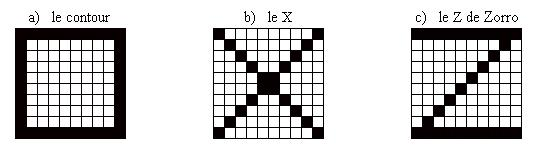
\includegraphics[width=0.7\textwidth]{image/tab2d-ex-oxz}
		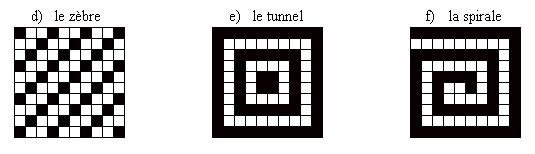
\includegraphics[width=0.7\textwidth]{image/tab2d-ex-zts}
		\end{center}
		
		Notes
		\begin{itemize}
		\item 
			Le zèbre doit toujours présenter des lignes
			obliques et parallèles, quelle que soit la taille.
		\item
			La spirale est un véritable défi
			et vous est donné comme exercice facultatif.
			Ne le faites pas si vous êtes en retard.
		\end{itemize}
	\end{Exercice}

	\begin{Solution}
		\begin{algo}
                  \Algo{pinceauZebre}{\Par{tab\InOut}{\Array{n $\times$ n}{entiers}}}{}{
                    \Assign{colDepart}{0}\;
                    \Fori[]{lg}{0}{n-1}{
                      \Fori[3]{col}{colDepart}{n-1}{
                        \Assign{tab[lg,col]}{NOIR}\;
                      }
                      \eIf{colDepart > 0 }{
                        \Assign{colDepart}{colDepart - 1}\;

                      }{
                        \Assign{colDepart}{2}\;
                      }

                    }
                  }
                  \Algo{pinceauSpirale}{\Par{tab\InOut}{\Array{n $\times$ n}{entiers}}}{}{
                    \Assign{lg}{0}\;
                    \Assign{col}{0}\;
                    \Assign{dirLg}{0}\;
                    \Assign{dirCol}{1}\;
                    \Assign{fini}{faux}\;
                    \While{NON fini}{
                      \Assign{tab[lg,col]}{NOIR}\;
                      \If{bord(lg,col,dirLg, dirCol) OU noircieDansDeuxCase(tab, lg,col,dirLg,dirCol) }{
                        tournerADroite(dirLg, dirCol)\;
                      }
                      avancer(lg, col, dirLg, dirCol)\;
                      \If{caseNoireADroite(tab,lg,col,dirLg, dirCol) }{
                        \Assign{fini}{vrai}\;

                      }
                    }
                  }
                  \Algo{bord}{\Par{lg, col, dirLg, dirCol}{entiers}}{booléen}{
                    \Assign{tmpLg}{lg}\;
                    \Assign{tmpCol}{col}\;
                    avancer(tmpLg, tmpCol, dirLg, dirCol)\;
                    \Return NON (0 <= tmpCol ET tmpCol < n ET 0 <= tmpLg ET tmpLg < n) \;
                  }
                  \Algo{noircieDansDeuxCase}{\Par{tab, lg, col, dirLg, dirCol}{entiers}}{booléen}{
                    \Assign{tmpLg}{lg}\;
                    \Assign{tmpCol}{col}\;
                    avancer(tmpLg, tmpCol, 2*dirLg, 2*dirCol)\;
                    \Return tab[tmpLg, tmpCol] == NOIR
                    \;
                  }
                \end{algo}
                \begin{algo}
                  \Algo{tournerADroite}{\Par{dirLg\InOut}{entier}, \Par{dirCol\InOut}{entier}}{}{
                    \Assign{dirLg}{dirCol}\;
                    \Assign{dirCol}{-dirLg}\;
                  }
                  \Comment{Tests: tournerADroite(0, 1) = (1, 0)}\;
                  \Comment{tournerADroite(1, 0) = (0, -1)}\;
                  \Comment{tournerADroite(0, -1)= (-1, 0)}\;
                  \Comment{tournerADroite(-1, 0)= (0, 1)}\;
                  \Algo{avancer}{\Par{lg\InOut}{entier}, \Par{col\InOut}{entier}, \Par{dirLg, dirCol}{entiers}}{}{
                    \Assign{lg}{lg + dirLg}\;
                    \Assign{col}{col + dirCol}\;
                  }
                  \Algo{caseNoireADroite}{\Par{tab, lg, col, dirLg, dirCol}{entiers}}{booléen}{
                    \Assign{tmpLg}{lg}\;
                    \Assign{tmpCol}{col}\;
                    \Assign{tmpDirLg}{dirLg}\;
                    \Assign{tmpDirCol}{dirCol}\;
                    tournerADroite(tmpDirLg, tmpDirCol)\;
                    \eIf{NON bord(lg,col, tmpDirLg, tmpDirCol) }{
                      avancer(tmpLg, tmpCol, dirLg, dirCol)\;
                      \Return  tab[tmpLg, tmpCol] = NOIR \;
                    }{
                      \Return  faux \;
                    }
                  }
		\end{algo}
	\end{Solution}
	
	\begin{Exercice}{Exercices sur la complexité}	
		Quelle est la complexité 
		\begin{enumerate}[label=\alph*)]
		\item 
			d’un algorithme de parcours	d'un tableau $n$ x $n$ ?
		\item
			des algorithmes que vous avez écrits pour les exercices :
			"Les nuls", "Tous positifs", "Le carré magique"
			et "Le contour d'un tableau" ?
		\item 
			des algorithmes que vous avez écrits pour résoudre les
			exercices du pinceau ?
		\end{enumerate}
	\end{Exercice}

	%========================
\chapter{L'orienté objet}
%=========================

	\marginicon{objectif}
	Le cours de Java vous a présenté la programmation orienté objet.
	Dans ce chapitre, nous allons rapidement revoir ce sujet
	et présenter comment nous allons l'utiliser dans ce cours.
	Nous nous contenterons de parler d'\textit{encapsulation}. 
	Les autres piliers de l'orienté objet 
	(\textit{héritage} et \textit{polymorphisme}) 
	ne seront pas vus cette année.

%===================
\section{Motivation}
%====================

	Au cours de Java,
	vous avez vu que l'orienté objet permet de structurer une
	application en regroupant dans un même \emph{objet}
	des données et le code qui va manipuler ces données.
	
	Une autre façon de voir l'orienté objet
	est de constater qu'une classe permet de définir 
	un nouveau \emph{type de données}.
	La notion de \emph{structure} permet déjà cela mais de façon limitée
	car elle ne reprend que des données et pas du code.
	Avec l'orienté objet, 
	on dispose de méthodes définissant ce qu'on peut faire avec des données
	(les objets) de ce type.
	C'est ainsi que nous l'utiliserons pour définir les listes 
	dans un prochain chapitre.

	
%=======================================
\section{Illustration~: une durée}
%=======================================

	Voyons tout cela au travers d'un exemple complet.
	Il est parfois utile d'avoir à sa disposition un type
	de données permettant de représenter une durée.	
	Utiliser plusieurs entiers (un pour les heures, un autre pour les minutes,
	un autre encore pour les secondes) n'est pas pratique.
	Utiliser une structure est déjà mieux mais offre moins d'avantage
	que l'orienté objet.	
	Voyons comment définir ce nouveau type de données en orienté objet.
	
	\subsection{Ce que l’on veut vraiment}
	%=====================================
	
		Avant tout, il faut bien préciser ce que l’on veut décrire
		et bien faire la distinction entre un \emph{moment} et une \emph{durée}.
		L’«~heure~» est un concept multifacette. 
		Parle-t-on de l’heure comme moment dans la journée 
		ou de l’heure comme représentant une durée ? 
		Dans le premier cas, elle ne peut dépasser 24h 
		et la différence entre 2 heures n’a pas de sens 
		(ou plus précisément n’est pas une heure, mais une durée !).
		Ce que nous nous proposons de créer ici est une durée,
		correspondant au deuxième cas.
		Et pour être plus précis encore,
		nous allons nous limiter à une précision à la seconde près,
		pas plus%
		\footnote{%
			Ajouter plus de précision ne serait pas plus compliqué à faire.%
		}.
	
	\subsection{Le comportement (les méthodes)}
	%==========================================
	
		La première question à se poser est celle des services que l’on veut
		fournir, c’est-à-dire des méthodes publiques de la classe. On doit
		pouvoir \textit{construire} une durée. On doit pouvoir connaitre le
		nombre de jours, d’heures, minutes ou secondes correspondant à une durée. On doit
		pouvoir effectuer des calculs avec des durées (addition, soustraction).
		Enfin, on doit pouvoir comparer des durées. Arrêtons-nous là, mais en
		pratique, on pourrait trouver encore bon nombre d’autres méthodes qu’il
		serait intéressant de fournir. 
		
		Voici comment nous allons noter tout cela au cours d'algorithmique.
		
		\begin{LDA}
			\Class{Durée}
				%\Private
					%\LComment rien encore
				\Public
					\ConstrSign{Durée}{secondes~: entier}
					\ConstrSign{Durée}{heure, minute, seconde~: entiers}
					\Empty
					\MethodSign{getJour}{}{entier}
					\RComment nb de jours dans une durée
					\MethodSign{getHeure}{}{entier}
					\RComment entier entre 0 et 23 inclus
					\MethodSign{getMinute}{}{entier}
					\RComment entier entre 0 et 59 inclus
					\MethodSign{getSeconde}{}{entier}
					\RComment entier entre 0 et 59 inclus
					\Empty
					\MethodSign{getTotalHeures}{}{entier}
					\RComment Le nombre total d’heures
					\MethodSign{getTotalMinutes}{}{entier}
					\RComment Le nombre total de minutes
					\MethodSign{getTotalSecondes}{}{entier}
					\RComment Le nombre total de secondes
					\Empty
					\MethodSign{ajouter}{autreDurée~: Durée}{}
					\MethodSign{différence}{autreDurée~: Durée}{Durée}
					%\MethodSign{égale}{autreDurée~: Durée}{booléen}
					\MethodSign{plusPetit}{autreDurée~: Durée}{booléen}
			\EndClass
		\end{LDA}
		
		\marginicon{attention}
		\textbf{Quelques remarques}
		\begin{itemize}
			\item
				On a deux constructeurs, ce qui offre plus de souplesse pour initialiser un objet. 
				On parle de «\textbf{~surcharge~}» des constructeurs.
			\item
				Faisons bien la distinction entre les méthodes
				\lda{getXXX()} et \lda{getTotalXXX()}. Par
				exemple, la méthode \lda{getMinute()} retourne la valeur
				de la composante «~minutes~» dans une représentation HMS tandis que la
				méthode \lda{getTotalMinutes()} retourne le nombre total
				de minutes entières pour cette durée. Ex~: pour 1h23’12’’,
				\lda{getMinute()} retourne 23 et
				\lda{getTotalMinutes()} retourne 83. 
				Idem avec les heures et les secondes.
			\item 
				Les méthodes \lda{getTotalXXX()} retournent le nombre
				(toujours entier) de XXX contenus dans la durée. Exemple, avec la durée
				0h23’52’’, \lda{getTotalMinutes()}
				retourne 23 et pas 24 (autrement dit, il n’y a pas d’arrondi vers le
				haut).
			\item 
				Il n’y a pas de \textit{mutateur} (\lda{setXXX()}). 
				Ce qui signifie qu’on ne peut pas changer directement la valeur de l’objet
				après son initialisation. 
				Les seules modifications viendront de la méthode \lda{ajouter()}.
				On aurait pu définir des mutateurs mais nous
				n'avons pas jugé utile de le faire dans ce cas précis.
				Vous verrez dans le cours de Java des motivations à ce choix.
			\item 
				La méthode \lda{ajouter()} ne retourne rien. En effet,
				elle ajoute la durée à l’objet sur lequel est appelée la méthode. C’est
				un choix ; on aurait aussi pu dire que la méthode ne modifie pas
				l’objet mais en retourne un autre qui représente la somme. Dans ce cas,
				on l’aurait plutôt appelée «\lda{~plus( )}~».
			\item 
				La méthode \lda{différence()}, elle, renvoie toujours une
				durée (positive).
			\item 
				Nous ne définissons pas de méthode d'affichage
				similaire au \lda{toString()} qu'on retrouve en Java.
				L'affichage correct de l'information ne fait pas partie
				des préoccupations de ce cours.
				On supposera que "\lda{\K{afficher} objet}"
				affiche correctement les données associées à l'objet.
		\end{itemize}
	
	\subsection{La représentation de l'état (les attributs)}
	%=======================================================
	
		La question suivante est~: «~Comment représenter une durée en interne ?
		». Plusieurs possibilités existent. Par exemple~:	
		\begin{itemize}
			\item 
				via le nombre d’heures, de minutes et de secondes
			\item 
				via le nombre total de secondes
			\item 
				via une chaine, par exemple au format «~HH~:~MM~:~SS~» où HH pourrait
				éventuellement excéder 23.
		\end{itemize}
		
		Le premier choix semble le plus évident mais réfléchissons-y de plus
		près. D’une part, pourquoi se limiter aux heures. On pourrait
		introduire un champ ‘\lda{jour}’ (après tout on a bien
		une méthode \lda{getJour()}). 		
		Quel critère doit vraiment nous permettre de décider ? Il faut une
		représentation qui soit suffisante (tout est représenté) et qui
		permette d’écrire des méthodes lisibles et si possible efficaces
		(c'est-à-dire où le calcul est rapide). Selon ces
		critères, la deuxième représentation est de loin la meilleure. 
		
		Voilà comment nous indiquons les attributs d'une classe.
		
		\begin{LDA}
			\Class{Durée}
				\Private
					\Decl{totalSecondes}{entier}
				\Public
					\LComment Ici viennent les constructeurs et les méthodes
			\EndClass
		\end{LDA}
	
		Pour rappel de votre cours de langage,
		ce qui est privé n'est pas utilisable directement 
		par du code extérieur à la classe.
		Un code extérieur, manipulant des objets de cette classe,
		ne peut utiliser que ce qui est public.
		
	\subsection{L'implémentation}
	%============================
	
		On est à présent prêt pour écrire le code des méthodes. 
		Pour une meilleure lisibilité,
		nous gardons les signatures des méthodes dans la classe
		et nous détaillons leur contenu en dehors.
		Ce qui donne :
		
		\begin{LDA}
			\Class{Durée}
				\Private
					\Decl{totalSecondes}{entier}
				\Public
					\ConstrSign{Durée}{secondes~: entier}
					\ConstrSign{Durée}{heure, minute, seconde~: entiers}
					\Empty
					\MethodSign{getJour}{}{entier}
					\RComment nb de jours dans une durée
					\MethodSign{getHeure}{}{entier}
					\RComment entier entre 0 et 23 inclus
					\MethodSign{getMinute}{}{entier}
					\RComment entier entre 0 et 59 inclus
					\MethodSign{getSeconde}{}{entier}
					\RComment entier entre 0 et 59 inclus
					\Empty
					\MethodSign{getTotalHeures}{}{entier}
					\RComment Le nombre total d’heures
					\MethodSign{getTotalMinutes}{}{entier}
					\RComment Le nombre total de minutes
					\MethodSign{getTotalSecondes}{}{entier}
					\RComment Le nombre total de secondes
					\Empty
					\MethodSign{ajouter}{autreDurée~: Durée}{}
					\MethodSign{différence}{autreDurée~: Durée}{Durée}
					%\MethodSign{égale}{autreDurée~: Durée}{booléen}
					\MethodSign{plusPetit}{autreDurée~: Durée}{booléen}
			\EndClass
		\end{LDA}

		\begin{LDA}
			\Constr{Durée}{secondes~: entier}
				\If{secondes < 0}
					\Stmt \K{erreur} "paramètre négatif"%
					\footnote{%
						L'instruction \K{erreur} indique
						que l'algorithme ne peut pas poursuivre normalement.
						Il s'arrête avec un message d'erreur.
					}					
				\EndIf
				\Let totalSecondes \Gets secondes
			\EndConstr
		\Empty
			\Constr{Durée}{heure, minute, seconde~: entiers}
				\If{heure < 0 OU minute < 0 OU seconde < 0 OU minute>59 ou seconde>59}
					\Stmt \K{erreur} "un des paramètres est invalide"
				\EndIf
				\Let totalSecondes \Gets 3600*heure + 60*minute + seconde
			\EndConstr
		\Empty
			\LComment Retourne le nombre de jours dans une 
			représentation JJ/HH:MM:SS
			\Method{getJour}{}{entier}
				\Return totalSecondes DIV (3600*24)
			\EndMethod
		\Empty
			\LComment Retourne le nombre d'heures dans une 
			représentation JJ/HH:MM:SS
			\Method{getHeure}{}{entier}
				\LComment On doit enlever les jours éventuels
				\Return (totalSecondes DIV 3600) MOD 24
			\EndMethod
		\Empty
			\LComment Retourne le nombre de minutes dans une 
			représentation JJ/HH:MM:SS
			\Method{getMinute}{}{entier}
				\LComment On doit enlever les heures éventuelles
				\Return (totalSecondes DIV 60) MOD 60
			\EndMethod
		\Empty
			\LComment Retourne le nombre de secondes dans une 
			représentation JJ/HH:MM:SS
			\Method{getSeconde}{}{entier}
				\LComment On doit enlever les minutes éventuelles
				\Return totalSecondes  MOD 60
			\EndMethod
		\Empty
			\LComment Retourne le nombre entier d’heures complètes
			\Method{getTotalHeures}{}{entier}
				\Return totalSecondes DIV 3600
			\EndMethod
		\Empty
			\LComment Retourne le nombre entier de minutes complètes
			\Method{getTotalMinutes}{}{entier}
				\Return totalSecondes DIV 60
			\EndMethod
		\Empty
			\LComment Retourne le nombre entier de secondes complètes
			\Method{getTotalSecondes}{}{entier}
				\Return totalSecondes
			\EndMethod
		\Empty
			\Method{ajouter}{autreDurée~: Durée}{}
				\Let totalSecondes \Gets totalSecondes + autreDurée.totalSecondes
			\EndMethod
		\Empty
			\Method{différence}{autreDurée~: Durée}{Durée}
				\Return \K{nouvelle} Durée(valeurAbsolue(totalSecondes - autreDurée.totalSecondes))
			\EndMethod
		%\Empty
			%\Method{égale}{autreDurée~: Durée}{booléen}
				%\Return totalSecondes = autreDurée.totalSecondes
			%\EndMethod
		\Empty
			\Method{plusPetit}{autreDurée~: Durée}{booléen}
				\Return totalSecondes < autreDurée.totalSecondes
			\EndMethod
		\end{LDA}
	
	%=====================================
	\subsection{Utilisation}
	%=====================================

		Pour utiliser le nouveau type de donnée créé,
		il faut l'instancier, c'est-à-dire créer un nouvel objet de ce type.
		Nous allons utiliser le mot clé \K{nouveau}
		(ou \K{nouvelle} si vous jugez utile d'accorder avec le type)
		pour rester très proche de Java.
		
		Illustrons cela au travers d'un petit algorithme
		qui calcule la différence entre deux durées.
		
		\begin{LDA}
			\Algo{diffDurée}{}{}
				\Decl{durée1, durée2}{Durée}	\RComment Les variables sont déclarées/créées
				\Let durée1 \Gets \K{nouvelle} Durée(3, 4, 49)	\RComment Les objets sont créés
				\Let durée2 \Gets \K{nouvelle} Durée(3, 24, 37)	\RComment Les objets sont créés
				\Write durée2.différence(durée1)
			\EndAlgo
		\end{LDA}

%=====================================
\section{Quelques éléments de syntaxe}
%=====================================

	Clarifions certaines notations liées aux objets.

	\begin{itemize}
		\item
			Pour un attribut \lda{brol},
			on choisira de nommer l'accesseur%
			\footnote{%
				Pour rappel,
				un \emph{accesseur} est une méthode 
				donnant la valeur d'un attribut.
			} \lda{getBrol}
			et le mutateur%
			\footnote{%
				Pour rappel,
				un \emph{mutateur} est une méthode 
				permettant de modifier la valeur d'un attribut.
			} \lda{setBrol}.
			Dans le cas particulier d'un attribut booléen,
			on pourra appeler l'accesseur \lda{isBrol} ou encore \lda{estBrol}.
		\item
			On peut directement afficher un objet. 
			Cela affiche l'état d'un objet d'une façon claire pour l'utilisateur%
			\footnote{%
				Le format précis n'est pas spécifié car il n'est pas important pour ce cours.
			}.

			\begin{LDA}
				\Decl{rendezVous}{Durée}
				\Let rendezVous \Gets \K{nouvelle} Durée(14, 23, 56)
				\Write rendezVous 
				\RComment affichera 14, 23 et 56 dans un format lisible.
			\end{LDA}
		\item
			De même, on peut directement lire un objet,
			ce qui a pour effet de créer un objet avec un état
			correspondant aux valeurs lues pour ses attributs.

			\begin{LDA}
				\Decl {rendezVous}{Durée}
				\Read rendezVous
			\end{LDA}
		\item 
			La comparaison de deux objets est toujours un problème délicat en orienté objet.
			Nous nous baserons ici sur les conventions \bsc{Java}
			et utiliserons la notation \lda{o1.égale(o2)}
			quand il s'agira de vérifier que \lda{o1} et \lda{o2} sont dans le même état,
			c'est-à-dire que leurs attributs ont la même valeur.
		\item
			Lorsqu'on déclare un objet, il n'est pas encore créé.
			On peut utiliser la valeur spéciale «~rien~»
			pour indiquer ou tester qu'un objet n'est pas encore créé.
			
			\begin{LDA}
				\Decl{parcours}{Durée}								\RComment parcours = rien
				\Let parcours \Gets \K{nouvelle} Durée( 14, 23, 56 )	\RComment parcours ${\neq}$ rien
				\If{parcours $\neq$ rien}
					\Let parcours \Gets rien						\RComment parcours = rien
				\EndIf
			\end{LDA}
		\item
			Si une classe ne propose pas de constructeur,
			on peut néanmoins instancier un objet 
			(via \lda{\K{nouveau} NomClasse()}).
			On considère dans ce cas que les attributs ne sont pas initialisés.
	\end{itemize}

\clearpage	
%==================================================
\section{Mise en pratique : le lièvre et la tortue}
%==================================================

	Partons d'un petit jeu, \og{}Le lièvre et la tortue\fg{}%
	\footnote{%
		Lu sur le net : 
		\url{http://mathemathieu.free.fr/2b/doc/pb_algo/problemes_et_algorithmique.pdf}
	}, 
	et voyons comment le coder en OO.

	\subsection{Description du jeu}
	%==============================
	
		Un lièvre et une tortue font une course.
		Le lièvre est plus rapide que la tortue.
		Pour donner plus de chance à la tortue de gagner une course de 5 km, 
		on adopte la règle de jeu suivante~:
		\begin{itemize}
		\item 
			On lance un dé. 
		\item
			Si le 6 sort, 
			le lièvre est autorisé à démarrer et gagne la course; 
			sinon on laisse la tortue avancer d’un kilomètre.
		\item
			On recommence le procédé jusqu'à la victoire du lièvre ou de la tortue.
		\end{itemize}
		
	\subsection{Solution non orientée objet}
	%=======================================
	
		Pour ne pas aller trop vite et vous perdre tout de suite,
		commençons par une version non orientée objet du jeu.
		
		\subsubsection*{Représenter le jeu}
		%----------------------------------	

			Il faut d'abord se poser cette question :
			Comment représenter le jeu ?
			Une représentation du jeu doit être complète.
			C'est-à-dire qu'à partir de cette représentation,
			on doit pouvoir indiquer exactement où on en est dans le jeu
			et pouvoir le poursuivre.
			
			Pour le dire autrement, 
			imaginons qu'on joue à ce jeu \og{}en vrai\fg{}, sur une table de jeu.
			La représentation informatique doit capturer tout ce qui est pertinent
			dans le jeu physique de sorte que, si on range la boite de jeu,
			on peut, le lendemain, reconstruire le jeu exactement comme il était.
			
			Dans notre exemple, cela veut dire quoi ?
			\begin{description}
			\item[La tortue]
				On doit pouvoir savoir où elle en est dans son avancée.
				Un petit entier (de 0 à 5) reprenant son avancée en km suffit.
				Appelons-le \lda{avancéeTortue} par exemple.
			\item[Le lièvre]
				Pendant le jeu, il est en permanence au départ
				et lorsque sort un 6, il atteint directement l'arrivée.
				Plusieurs possibilités s'offrent à nous :
			
				\begin{enumerate}
				\item
					On pourrait imaginer un entier valant 0 ou 5,
					appelé \lda{avancéeLièvre}.
				\item
					On pourrait aussi imaginer un booléen à vrai 
					lorsqu'il est au départ et faux lorsqu'il est à l'arrivée.
					On pourrait l'appeler \lda{lièvreAuDépart}.
				\item
					Ou encore un booléen ayant exactement le sens inverse.
					Le nom devra être choisi judicieusement pour ne pas induire
					le lecteur en erreur.
					Par exemple, ici, on pourrait choisir \lda{lièvreArrivé}.
				\end{enumerate}
				
				Ici, le troisième choix nous semble le plus pertinent.
			\item[Le dé]
				Un entier de 1 à 6 suffit pour représenter le résultat d'un dé.
				Appelons-le simplement \lda{dé}.
			\item[Les joueurs]
				Si on observe un jeu physique,
				on peut s'attarder sur les personnes en train de jouer.
				Faut-il les représenter ?
				On pourrait imaginer de connaitre leur nom,
				le nombre de fois qu'elles ont joué à ce jeu,
				leur nombre de victoires.
				Dans l'énoncé, 
				rien n'indique qu'il faille tenir compte de tout cela. 
				On s'intéresse au jeu proprement dit, et c'est tout.
			\item[Le plateau]
				On peut imaginer que dans le jeu physique,
				il y aurait une sorte de plateau 
				avec des km indiqués
				sur lequel avancerait la tortue.
				Mais il n'y a aucune information changeante
				sur ce plateau qui vaille la peine d'être retenue.
			\end{description}

		\subsubsection*{Un macro algorithme}
		%----------------------------------	
				
			Avant de se lancer dans l'écriture d'une solution détaillée du jeu,
			commençons par une solution non détaillée
			et voyons si tout semble clair et faisable.
			
			\begin{LDA}
				\Algo{jeuLièvreTortue}{}{}
					\Stmt Initialiser le jeu
					\While{le jeu n'est pas fini}
						\Stmt{Lancer le dé}
						\If{le dé est 6}
							\Stmt Le lièvre est arrivé
						\Else
							\Stmt La tortue avance
						\EndIf
						\Write l'état du jeu
					\EndWhile
					\Write le vainqueur
				\EndAlgo
			\end{LDA}
			
		\subsubsection*{Détailler l'algorithme}
		%----------------------------------	
	
			Repassons à présent sur l'algorithme
			et vérifions que nous pouvons détailler 
			chacun des points restés généraux.
			\begin{itemize}
			\item \textbf{Initialiser le jeu.}
				Il suffit de placer la tortue en 0
				et d'indiquer que le lièvre n'est pas encore arrivé.
				La valeur initiale du dé n'a pas d'importance.
			\item \textbf{Le jeu n'est pas fini.}
				Le jeu sera fini lorsque le lièvre sera arrivé
				(ce qu'on peut tester grâce au booléen \lda{lièvreArrivé})
				ou que la tortue sera au km 5.
			\item \textbf{Lancer le dé.}
				C'est trivial si on utilise l'algorithme \lda{hasard()}
				à notre disposition.
			\item \textbf{Le lièvre est arrivé.}
				Il suffit de mettre le booléen \lda{lièvreArrivé} à vrai.
			\item \textbf{La tortue avance.}
				C'est trivial.
			\item \textbf{Afficher l'état du jeu.}
				À savoir, sur quelle face est tombé le dé
				et où se trouvent à présent le lièvre et la tortue.
			\item \textbf{Afficher le vainqueur.}
				Ce sera le lièvre si son booléen est à vrai et la tortue sinon
				(dans ce cas, son avancée sera forcément de 5 
				puisque le jeu est fini).
			\end{itemize}
			
			Au final, on obtient :
			\begin{LDA}
				\Algo{jeuLièvreTortue}{}{}
					\Decl{avancéeTortue}{entier}
					\Decl{lièvreArrivé}{booléen}
					\Decl{dé}{entier}

					\Empty
					\Let avancéeTortue \Gets 0
					\Let lièvreArrivé \Gets faux
					
					\Empty
					\While{avancéeTortue < 5 ET NON lièvreArrivé}
						\Let dé \Gets hasard(6)
						\If{dé = 6}
							\Let lièvreArrivé \Gets vrai
						\Else
							\Let avancéeTortue \Gets avancéeTortue + 1
						\EndIf
						\Write dé, avancéeTortue, lièvreArrivé
					\EndWhile

					\Empty
					\If{lièvreArrivé}
						\Write "Le lièvre a gagné"
					\Else
						\Write "Le tortue a gagné"
					\EndIf
				\EndAlgo
			\end{LDA}

	\subsection{Solution orientée objet}
	%=======================================
		
		Voyons à présent ce que ça pourrait donner si on introduit
		de l'orienté objet.
		Examinons d'abord les objets physiques du jeu.
		\begin{description}
		\item[La tortue]
			On peut envisager de définir une classe pour la tortue.
			Une tortue a une avancée. 
			Au départ, elle est au kilomètre 0.
			Elle peut avancer d'un kilomètre à la fois.
			Elle a fini et gagne lorsqu'elle arrive au kilomètre 5.

			\begin{LDA}
				\Class{Tortue}
				\Private
					\Decl{avancée}{entier}
				\Public
					\Constr{Tortue}{}
						\Let avancée \Gets 0						
					\EndConstr
					\Empty
					\Method{avancer}{}{}
						\Let avancée \Gets avancée + 1						
					\EndMethod
					\Empty
					\Method{estArrivée}{}{booléen}
						\Return avancée = 5
					\EndMethod
					\Empty
					\Method{getAvancée}{}{entier}
						\Return avancée
					\EndMethod
				\EndClass
			\end{LDA}

			Remarquez qu'on n'introduit pas de mutateur
			car on veut que la tortue n'avance qu'en respectant les
			règles du jeu.

\clearpage

		\item[Le lièvre]
			On peut appliquer la même démarche pour le lièvre
			qui aurait un attribut booléen indiquant s'il est arrivé ou pas.

		\item[Le dé]		
			Le dé est également un objet de notre jeu
			et peut être défini via une classe.

			\begin{minipage}{6cm}
			\begin{LDA}
				\Class{Lièvre}
				\Private
					\Decl{arrivé}{booléen}
				\Public
					\Constr{Lièvre}{}
						\Let arrivé \Gets faux					
					\EndConstr
					\Empty
					\Method{avancer}{}{}
						\Let arrivé \Gets vrai
					\EndMethod
					\Empty
					\Method{estArrivé}{}{booléen}
						\Return arrivé
					\EndMethod
				\EndClass
			\end{LDA}
			\end{minipage}
			~
			\begin{minipage}{6cm}
			\begin{LDA}
				\Class{Dé}
				\Private
					\Decl{valeur}{entier}
				\Public
					\Constr{Dé}{}
					\EndConstr
					\Empty
					\Method{lancer}{}{}
						\Let valeur \Gets hasard(6)
					\EndMethod
					\Empty
					\Method{getValeur}{}{entier}
						\Return valeur
					\EndMethod
				\EndClass
			\end{LDA}
			\end{minipage}

		\end{description}

		\subsubsection*{L'algorithme du jeu}
		%-----------------------------------
		
			L'algorithme du jeu peut être récrit
			en utilisant les trois classes qu'on vient de définir.
			
			\begin{LDA}
				\Algo{jeuLièvreTortue}{}{}
					\Decl{tortue}{Tortue}
					\Decl{lièvre}{Lièvre}
					\Decl{dé}{Dé}

					\Empty
					\Let tortue \Gets \K{nouvelle} Tortue()
					\Let lièvre \Gets \K{nouveau} Lièvre()
					\Let dé \Gets \K{nouveau} Dé()
					
					\Empty
					\While{NON tortue.estArrivée() ET NON lièvre.estArrivé()}
						\Stmt dé.lancer()
						\If{dé.getValeur()=6}
							\Stmt lièvre.avancer()
						\Else
							\Stmt tortue.avancer()
						\EndIf
						\Write dé.getValeur(), tortue.getAvancée(), lièvre.estArrivé()
					\EndWhile

					\Empty
					\If{lièvre.estArrivé()}
						\Write "Le lièvre a gagné"
					\Else
						\Write "Le tortue a gagné"
					\EndIf
				\EndAlgo
			\end{LDA}
			
			Est-ce une bonne idée d'avoir défini ces trois classes ?
			C'est une question qu'il est légitime de se poser
			quand les classes sont aussi simples.
			Remarquons toutefois que le code est plus modulaire
			et que la méthode principale est plus facile à lire.
			
			La classe \lda{Dé} se justifie d'autant plus 
			qu'elle pourra probablement servir à de nombreuses occasions.
			Ce sera encore plus le cas
			si on la généralise à des dés qui n'ont pas forcément 6 faces.

			\begin{LDA}
				\Class{Dé}
				\Private
					\Decl{nbFaces}{entier}
					\Decl{valeur}{entier}
				\Public
					\Constr{Dé}{\Par{nf}{entier}}
						\Let nbFaces \Gets nf
					\EndConstr
					\Empty
					\Method{lancer}{}{}
						\Let valeur \Gets hasard(nbFaces)
					\EndMethod
					\Empty
					\Method{getValeur}{}{entier}
						\Return valeur
					\EndMethod
				\EndClass
			\end{LDA}
			
			Dans l'algorithme principal,
			le seul changement est la création du dé qui devient :
			\begin{LDA}
					\Let dé \Gets \K{nouveau} Dé(6)
			\end{LDA}
				
	\subsection{Solution MVC (\og{}Modèle-Vue-Contrôleur\fg{})}
	%=======================================
		
		Dans la version OO qu'on vient de voir,
		on a introduit trois classes 
		mais il reste tout un morceau, l'algorithme principal, qui n'est pas OO.
		Peut-on aller plus loin dans l'OO ?
		Bien sûr ! 
		Mais il y a de bonnes et de mauvaises façons de le faire.
		
		La mauvaise approche 
		est de simplement mettre l'algorithme principal dans une classe.
		Ce qui donnerait :

		\begin{LDA}
			\Class{LièvreTortue}
				\Constr{LièvreTortue}{}
				\EndConstr
				\Empty
				\Method{jouer}{}{}
					\LComment Idem algorithme jeuLièvreTortue() ci-avant  
				\EndMethod
			\EndClass
		\end{LDA}
		
		Ce qui réduirait l'algorithme principal à :
		\begin{LDA}
			\Algo{jeuLièvreTortue}{}{}
				\Decl{jeu}{LièvreTortue}
				\Let jeu \Gets \K{nouveau} LièvreTortue()
				\Stmt jeu.jouer()
			\EndAlgo
		\end{LDA}
		ou même, en se passant de la variable locale :
		\begin{LDA}
			\Algo{jeuLièvreTortue}{}{}
				\Stmt (\K{nouveau} LièvreTortue()).jouer()
			\EndAlgo
		\end{LDA}

		Cette approche est correcte mais n'exploite en rien 
		les avantages de l'OO.
		Une meilleure idée est de suivre l'approche MVC
		que nous allons vous expliquer.
		
		Dans l'approche MVC,
		on découpe le code en différentes parties.
		La partie \og{}modèle\fg{} regroupe les bouts de code
		qui font vraiment quelque chose (on parle de \og{}métier\fg{})
		tandis que la partie \og{}vue\fg{} regroupe les bouts de code
		qui interagissent avec l'utilisateur (demandes et affichages).
		La partie \og{}contrôleur\fg{}, quant à elle,
		conserve le code qui fait le lien entre le modèle et la vue.
		
		Si on respecte cette approche, 
		le métier ne contient \textbf{aucune} interaction avec l'utilisateur
		et la vue ne s'occupe \textbf{que} de l'interaction avec l'utilisateur.
		Il y a là de nombreux avantages :
		\begin{itemize}
		\item
			Les compétences pour écrire le modèle
			(connaissance du métier, accès à des bases de données\dots)
			et le dialogue avec les utilisateurs 
			(ergonomie, graphisme\dots)
			ne sont pas les mêmes.
			On peut donc confier ces parties à des équipes spécialisées.
		\item
			On pourra facilement changer le dialogue avec l'utilisateur.
			Ainsi, si on possède une version console du jeu,
			il suffira, pour en faire une autre version 
			(console, graphique, web\dots)
			de recommencer la vue 
			(et probablement d'adapter le contrôleur)
			sans toucher au modèle.
		\end{itemize}
	
		\paragraph{Le modèle.}
		%---------------------
		Dans notre exemple, le modèle contiendrait les algorithmes suivants :
		\begin{itemize}
		\item
			Initialiser le jeu : 
			placer la tortue et le lièvre à leur position de départ.
		\item
			Jouer un coup : 
			lancer le dé et déplacer le lièvre ou la tortue.
		\item
			Tester si le jeu est fini ou pas.
		\item
			Trouver le vainqueur.
		\end{itemize}

		Chacun de ces algorithmes est implémenté par une méthode
		(sauf l'initialisation qui est du ressort du constructeur).
		Au niveau des attributs, 
		on retrouve les éléments du jeu : le lièvre, la tortue et le dé.
		\footnote{%
			Une autre façon de voir les choses
			est de dire qu'on trouve en attributs
			les variables locales de la version non OO
			qui sont partagées par les différentes méthodes.
			Ici, il s'agit de toutes les variables locales
			mais ce n'est pas toujours le cas.
			Le dé, par exemple, n'est un attribut que parce que
			la vue voudra le connaitre pour le montrer à l'utilisateur.
			Sans cela, il pourrait être une variable locale
			de la méthode \lda{jouerCoup()}.
		}
		
		Ce qui donne :
		\begin{LDA}
			\Class{LièvreTortue}
				\Private
					\Decl{tortue}{Tortue}
					\Decl{lièvre}{Lièvre}
					\Decl{dé}{Dé}
				\Public
					\ConstrSign{LièvreTortue}{}
					\MethodSign{estFini}{}{booléen}
					\MethodSign{jouerCoup}{}{}
					\MethodSign{getVainqueur}{}{chaine}
					\LComment
						+ les accesseurs (getLièvre, getTortue et getDé)
						des attributs mais pas les mutateurs
			\EndClass
		\end{LDA}
		
		\begin{LDA}
			\Constr{LièvreTortue}{}
				\Let tortue \Gets \K{nouvelle} Tortue()
				\Let lièvre \Gets \K{nouveau} Lièvre()
				\Let dé \Gets \K{nouveau} Dé(6)						
			\EndConstr				
			\Empty
			\Method{estFini}{}{booléen}
				\Return tortue.estArrivée() OU lièvre.estArrivé()
			\EndMethod
		\end{LDA}
		
		\begin{LDA}
			\Method{jouerCoup}{}{}
				\Stmt dé.lancer()
				\If{dé.getValeur()=6}
					\Stmt lièvre.avancer()
				\Else
					\Stmt tortue.avancer()
				\EndIf
			\EndMethod

			\Empty
			\Method{getVainqueur}{}{chaine}
				\If{lièvre.estArrivé()}
					\Return "Lièvre"
				\Else
					\Return "Tortue"
				\EndIf
			\EndMethod
		\end{LDA}
			
		\paragraph{La vue.}
		%---------------------
		Avec notre exemple, plutôt simple, il n'y a pas de lecture
		mais il reste des affichages :
		\begin{itemize}
		\item
			Afficher l'état du jeu après un coup : 
			valeur du dé et nouvelles positions du lièvre et de la tortue.
		\item
			Afficher le vainqueur.
		\end{itemize}
		
		Cet exemple est probablement trop simple pour nécessiter une classe%
		\footnote{
			Une erreur classique est de placer ces algorithmes
			dans les classes associées du modèle
			car cela contrevient à la règle : 
			aucune interaction utilisateur dans le modèle.
		}.
		On pourrait se contenter de deux algorithmes classiques.
		
		\begin{LDA}
			\Algo{afficherÉtat}{\Par{jeu}{LièvreTortue}}{}
				\Write jeu.getDé().getValeur()
				\Write jeu.getTortue().getAvancée()
				\Write jeu.getLièvre().estArrivé()
			\EndAlgo
			
			\Empty
			\Algo{afficherVainqueur}{\Par{jeu}{LièvreTortue}}{}
				\Write "Le gagnant est : ", jeu.getVainqueur()
			\EndAlgo
		\end{LDA}
		
		\paragraph{Le contrôleur.}
		%-------------------------
		
		Le contrôleur est ce qui n'a pas été placé dans la vue ou le modèle,
		c'est-à-dire le code qui crée la dynamique entre tous ces éléments.

		\begin{LDA}
			\Algo{jeuLièvreTortue}{}{}
				\Decl{jeu}{LièvreTortue}
				\Stmt jeu \Gets \K{nouveau} LièvreTortue()
				\While{NON jeu.estFini()}
					\Stmt jeu.jouerCoup()
					\Stmt afficherÉtat(jeu)
				\EndWhile
				\Stmt afficherVainqueur(jeu)
			\EndAlgo
		\end{LDA}
		
		Remarquez la concision et la lisibilité de ce qu'on vient d'écrire.

	%=================
\chapter{La liste}
%=================

	\marginicon{objectif}
	
	Imaginons qu’on désire manipuler par programme une liste de contacts ou
	encore une liste de rendez-vous. Cette liste va varier ; sa taille
	n’est donc pas fixée. Utiliser un tableau à cet effet n’est pas l’idéal. 
	En effet, la taille d’un tableau ne peut plus changer une fois le tableau créé. 
	Il faudrait le surdimensionner, ce qui n’est pas économe.
	
	Il serait intéressant de disposer d’une structure qui offre toutes les
	facilités d’un tableau tout en pouvant «~grandir~» si nécessaire.
	Construisons une telle structure de données et appelons-la «~Liste~»
	pour rester en phase avec son appellation commune en Java.
	
	Par exemple, considérons une liste de courses.
	On pourrait la représenter ainsi :
	\begin{enumerate}
	\item "fromage"
	\item "pain"
	\item "salami"
	\end{enumerate}
	
	On pourrait ajouter un élément en fin de liste, par exemple de l'eau,
	pour obtenir la liste :
	
	\begin{enumerate}
	\item "fromage"
	\item "pain"
	\item "salami"
	\item "eau"
	\end{enumerate}
	
	On pourrait aussi supprimer un élément de la liste, par exemple le pain,
	et obtenir :
	
	\begin{enumerate}
	\item "fromage"
	\item "salami"
	\item "eau"
	\end{enumerate}
	
	On pourrait aussi insérer un élément dans la liste, 
	par exemple une baguette, 
	ce qui décale, de facto, la position des suivants.
	
	\begin{enumerate}
	\item "fromage"
	\item "salami"
	\item "baguette"
	\item "eau"
	\end{enumerate}
	
	Et encore plein de choses que nous allons détailler.
	
	%========================
	\section{La classe Liste}
	%=========================
	
		Nous verrons plus loin comment réaliser une classe Liste en pratique 
		mais nous pouvons déjà définir le comportement qu’on en attend 
		(les méthodes qu’elle doit fournir).
		
		Ce comportement sera identique quel que soit le type des éléments
		de la liste; une liste de chaines et une liste d'entiers
		ne se distinguent que par le type de certains paramètres
		et valeurs de retour.
		Ici, nous indiquons \lda{T} pour indiquer un type quelconque;
		vous pouvez le remplacer par ce qui vous convient : 
		entier, chaine, Date\dots
		
		\begin{LDA}
			\Class{Liste de T}
				\RComment T est un type quelconque
				\Private
					\LComment sera complété plus tard	
				\Public
					\ConstrSign{Liste de T}{}			
						\RComment construit une liste vide
					\MethodSign{get}{pos : entier}{T}
						\RComment donne un élément en position pos
					\MethodSign{set}{pos : entier, valeur : T}{}
						\RComment modifie un élément en position pos
					\MethodSign{taille}{}{entier}
						\RComment donne le nombre actuel d’éléments
					\MethodSign{ajouter}{valeur : T}{}
						\RComment ajoute un élément en fin de liste
					\MethodSign{insérer}{pos : entier, valeur : T}{}
						\RComment insère un élément en position pos
					\MethodSign{supprimer}{}{}
						\RComment supprime le dernier élément
					\MethodSign{supprimerPos}{pos : entier}{}
						\RComment supprime l'élément en position pos
					\MethodSign{supprimer}{valeur : T}{booléen}
						\RComment supprime l'élément de valeur donnée
					\MethodSign{vider}{}{}
						\RComment vide la liste
					\MethodSign{estVide}{}{booléen}
						\RComment la liste est-elle vide ?
					\MethodSign{existe}{valeur \In : T, pos \Out : entier}{booléen}
						\RComment recherche un élément
				\EndClass
		\end{LDA}
		
		\bigskip
		
		Quelques précisions s’imposent :
		\begin{itemize}
			\item 
				Les méthodes «\lda{~get~}» et «\lda{~set~}»
				permettent de connaitre ou modifier un élément de la liste. On
				considère, au cours d'algorithmique, que le premier élément de 
				la liste est en position 0.
			\item 
				«\lda{~ajouter~}» ajoute un élément en fin de liste (elle
				grandit donc d’une unité)
			\item 
				«\lda{~insérer~}» insère un élément à une position donnée
				(entre 0 et taille-1). L’élément qui s’y trouvait est décalé
				d'une position ainsi que tous les éléments suivants.
			\item 
				La méthode «\lda{~supprimerPos~}»
				supprime un élément d'une position donnée en
				décalant les éléments suivants. On pourrait imaginer une technique plus
				rapide consistant à placer le dernier élément à la place de l’élément
				supprimé mais ce faisant on changerait l’ordre relatif des éléments ce
				qui va à l’encontre de l’idée intuitive qu’on se fait d’une liste.
				Cette amélioration pourrait plutôt s’envisager dans une structure de
				type \textbf{ensemble} pour lequel il n’y a pas d’ordre relatif entre
				les éléments.
			\item 
				La version de «\lda{~supprimer~}» avec une valeur en
				paramètre enlève un élément de valeur donnée. Elle retourne un booléen
				indiquant si la suppression a pu se faire ou pas (ce qui sera le cas si
				la valeur n’est pas présente dans la liste). Si la valeur existe en
				plusieurs exemplaires, on prendra la convention arbitraire que
				la méthode n’en supprime que la première	occurrence.
			\item 
				La méthode «\lda{~existe~}» permet de savoir si un élément
				donné existe dans la liste. 
				\begin{itemize}
					\item 
						si c’est le cas, elle précise aussi sa position dans le paramètre sortant 
						\lda{pos}
					\item 
						si l’élément n’existe pas, ce paramètre est	indéterminé 
					\item 
						si l’élément est présent en plusieurs exemplaires, la méthode donne la
						position de la première occurrence.
				\end{itemize}
			\item 
				En pratique, il serait intéressant de chercher un élément à partir d’une
				partie de l’information qu’elle contient mais c’est difficile à
				exprimer de façon générique c'est-à-dire lorsque le
				type n'est pas connu à priori.
		\end{itemize}
		
		{\sffamily\bfseries\scshape
		Exemple : manipulations de base}
		
		Soit l'algorithme suivant :
		
		\begin{LDA}
			\Algo{ex1}{}{}
				\Decl{l}{Liste d'entiers}
				\Let l \Gets \K{nouvelle} Liste d'entiers()
				\Stmt l.ajouter(42)
				\Stmt l.ajouter(54)
				\Stmt l.set(1,44)
				\Stmt l.insérer(1,43)
				\Stmt l.supprimerPos(2)
				\Stmt l.supprimer(42)
				\Stmt l.vider
			\EndAlgo
		\end{LDA}
		
		Après sa création, la liste est vide.
		Ensuite, elle passe par les états suivants :
		
		\begin{minipage}[t]{2cm}
		\begin{enumerate}[start=0]
		\item 42
		\end{enumerate}
		\end{minipage}
		\begin{minipage}[t]{2cm}
		\begin{enumerate}[start=0]
		\item 42
		\item 54
		\end{enumerate}
		\end{minipage}
		\begin{minipage}[t]{2cm}
		\begin{enumerate}[start=0]
		\item 42
		\item 44
		\end{enumerate}
		\end{minipage}
		\begin{minipage}[t]{2cm}
		\begin{enumerate}[start=0]
		\item 42
		\item 43
		\item 44
		\end{enumerate}
		\end{minipage}
		\begin{minipage}[t]{2cm}
		\begin{enumerate}[start=0]
		\item 42
		\item 43
		\end{enumerate}
		\end{minipage}
		\begin{minipage}[t]{2cm}
		\begin{enumerate}[start=0]
		\item 43
		\end{enumerate}
		\end{minipage}
		
		Enfin, le dernier appel la vide complètement
		
		\bigskip
		{\sffamily\bfseries\scshape
		Exemple : recherche du minimum}
		
		Dans le chapitre sur les tableaux, vous avez fait un exercice consistant
		à afficher tous les indices où se trouve le minimum d’un tableau.
		Reprenons-le et modifions-le afin qu’il retourne la liste des indices
		où se trouvent les différentes occurrences du minimum. On pourrait
		l’écrire ainsi :
		
		\begin{LDA}
			\Algo{indicesMinimum}{\Par{tab}{\Array{n}{entiers}}}{Liste d'entiers}
				\Decl{min}{entier}
				\Decl{indicesMin}{Liste d'entiers}
				\Let min \Gets tab[0]
				\Let indicesMin \Gets \K{nouvelle} Liste d'entiers()
				\Stmt indicesMin.ajouter( 0 )
				\For{i}{1}{n-1}
					\If{tab[i] = min}
						\Stmt indicesMin.ajouter( i )
					\ElsIf{tab[i] < min}
						\Stmt indicesMin.vider() 
						\Stmt indicesMin.ajouter( i )
						\Let min \Gets tab[i]
					\EndIf \Comment rien à faire si tab[i] > min
				\EndFor
				\Return indicesMin
			\EndAlgo
		\end{LDA}
	
	%\clearpage
	%===================================
	\section{Comment implémenter l’état}
	%===================================
	
		Cette liste est bien utile mais comment la réaliser en pratique ?
		Comment représenter une liste variable d’éléments ? Pour
		l'instant, la seule structure qui peut accueillir
		plusieurs éléments de même type est le tableau. Nous allons donc
		prendre comme attribut principal de la liste un tableau que nous
		appellerons \lda{éléments}. Comment, dès lors, contourner
		le problème de la limitation de la taille de ce tableau ?
		
		Repartons donc de la notion de tableau et tentons de comprendre sa
		limitation. Lors de sa création, un tableau se voit attribuer un espace
		bien précis et contigu en mémoire. Il se peut très bien que
		l'espace «~juste après~» soit occupé par une autre
		variable ce qui l'empêche de grandir. La parade est
		claire : si un \ tableau s’avère trop petit lors de son utilisation, il
		suffit d’en créer un autre plus grand ailleurs en mémoire et d’y
		recopier tous les éléments du premier. Évidemment, cette opération est
		couteuse en temps et on cherchera à l’effectuer le moins souvent
		possible.
		
		\textbf{Quelle taille donner au nouveau tableau} ? L’idée qui vient
		immédiatement est d’augmenter la taille d’une unité afin d’accueillir
		le nouvel élément mais cette approche implique de fréquents
		agrandissements. Il est plus efficace d’augmenter la taille
		proportionnellement, par exemple en la multipliant par un facteur 2.
		
		\begin{center}
		\begin{tabular}{|m{0.259cm}|m{0.259cm}|m{0.259cm}|m{0.087999985cm}m{0.46000004cm}m{0.087999985cm}|m{0.25300002cm}|m{0.259cm}|m{0.259cm}|m{0.15299998cm}|m{0.15299998cm}|m{0.17cm}|}
		\hhline{---~~~------}
		 1 &
		 5 &
		 7 &
		~
		 &
		 ${\Rightarrow}$ &
		~
		 &
		 1 &
		 5 &
		 7 &
		 . &
		 . &
		 .\\\hhline{---~~~------}
		\end{tabular}
		\end{center}
		
		
		\textbf{Taille logique et taille physique}. À tout moment, le tableau
		aura une et une seule taille même si celle-ci pourra changer au cours
		du temps. Puisqu’on multipliera la taille du tableau par 2 pour des
		raisons d’efficacité, il y aura toutefois une différence entre la
		\textbf{taille physique} d’un tableau et sa \textbf{taille logique}. La
		taille physique est le nombre de cases réservées pour le tableau alors
		que la taille logique est le nombre de cases effectivement occupées.
		Dans ce qui suit, on s'arrangera pour que les cases
		occupées soient groupées à gauche du tableau (il n'y a
		pas de trou). Pour l’utilisateur, seule la taille logique a un sens (on
		lui cache les détails d’implémentation).
		
		\textbf{Exemple} : pour le tableau suivant, la taille logique est de 6
		(c’est cette taille qui a du sens pour l’utilisateur de la liste) et la
		taille physique est de 8.
		
		\begin{center}
		\begin{tabular}{|*{8}{>{\centering\arraybackslash}m{0.5cm}|}}
		\hline
		 2 &
		 5 &
		 4 &
		 8 &
		 3 &
		 12 &
		. &
		. \\\hline
		\end{tabular}
		\end{center}
		
		Quand il faut insérer un élément (en position valide) ou en ajouter un
		en fin de liste, deux cas se présentent :
		
		\begin{itemize}
			\item 
				si la taille logique est plus petite que la taille physique, il suffit
				d’ajouter l’élément dans le tableau et d’adapter la taille logique.
			\item 
				si la taille logique est égale à la taille physique, il faut
				procéder à un agrandissement du tableau.
		\end{itemize}
		
		\textbf{Les tableaux dynamiques}. 
		En \emph{DEV$_1$},
		nous n'avons vu que des tableaux
		qu'on appellera \emph{statiques},
		qui sont créés lors de leur déclaration.
		Ici, nous avons besoin de tableaux 
		qu'on appellera \emph{dynamiques},
		créés dans le code
		(comme le sont les tableaux en Java).
		
		Introduisons une notation.
		Un tableau dynamique sera déclaré puis créé ainsi :
		
			\begin{LDA}
				\Decl{tab}{\K{tableau} de chaines}
				\Let tab \Gets \K{nouveau} \Array{n}{chaines} \RComment n doit avoir une valeur
			\end{LDA}
		
		\textbf{Implémentation}.
		Présentons les attributs nécessaires et l'algorithme
		d’agrandissement du tableau.
		
		\begin{LDA}
			\Class{Liste de T}
				\Private
					\Decl{éléments}{\K{tableau} de T}
					\Decl{tailleLogique}{entier}
					\Decl{taillePhysique}{entier}
				\Private
					\Method {agrandir}{}{}
						\Decl{nouveauTab}{\K{tableau} de T}
						\Let taillePhysique \Gets taillePhysique * 2
						\Let nouveauTab \Gets \K{nouveau} \Array{taillePhysique}{T}
						\For{i}{0}{tailleLogique-1}
							\Let nouveauTab[ i ] \Gets éléments[ i ]
						\EndFor
						\Let éléments \Gets nouveauTab
					\EndMethod
				\EndClass
			\end{LDA}
		
		\bigskip
		
		\textbf{Réduction du tableau}. Tout comme on agrandit le tableau si
		nécessaire, on pourrait le réduire lorsque des suppressions d’éléments
		le rendent sous-utilisé (par exemple lorsque la taille logique devient
		inférieure au tiers de la taille physique). 
		Nous n'aborderons pas cette problématique cette année.
	
	
	%=======================================
	\section{Implémentation du comportement}
	%=======================================
	
		Nous avons à présent toutes les cartes en main pour écrire les méthodes
		publiques de la classe.
		
		\begin{LDA}
			\Constr{Liste de T}{}
				\Let tailleLogique \Gets 0
				\RComment la liste est vide au départ
				\Let taillePhysique \Gets 32
				\RComment une bonne valeur pour commencer
				\Let éléments \Gets \K{nouveau} \Array{taillePhysique}{T}
			\EndConstr
		\end{LDA}
		
		\begin{LDA}
			\Method{get}{pos : entier}{T}
				\If{ pos < 0 OU pos $\geq$ tailleLogique}
					\Error "position invalide"
				\EndIf
				\Return éléments[ pos ]
			\EndMethod
		\end{LDA}
		
		\begin{LDA}
			\Method{set}{pos : entier, valeur : T}{}
				\If{ pos < 0 OU pos $\geq$ tailleLogique}
					\Error "position invalide"
				\EndIf
				\Let éléments[ pos ] \Gets valeur
			\EndMethod
		\end{LDA}
		
		\begin{LDA}
			\Method{taille}{}{entier}
				\Return tailleLogique
				\RComment et pas la taille physique !
			\EndMethod
		\end{LDA}
		
		\begin{LDA}
			\Method{ajouter}{valeur : T}{}
				\If{tailleLogique = taillePhysique}
					\Stmt agrandir()
					\RComment méthode privée détaillée supra
				\EndIf
				\Let éléments[ tailleLogique ] \Gets valeur
				\Let tailleLogique \Gets tailleLogique + 1
			\EndMethod
		\end{LDA}
		
		\begin{LDA}
			\Method{insérer}{pos : entier, valeur : T}{}
				\If{ pos < 0 OU pos $\geq$ tailleLogique}
					\Error "position invalide"
				\EndIf
				\If{tailleLogique = taillePhysique}
					\Stmt agrandir()
				\EndIf
				\Stmt décalerDroite( pos )
				\RComment voir ci-dessous
				\Let tailleLogique \Gets tailleLogique + 1
				\Let éléments[ pos ] \Gets valeur
			\EndMethod
		\end{LDA}
		
		\begin{LDA}
			\Method{supprimer}{}{}
				\LComment supprime le dernier élément
				\If{tailleLogique = 0}
					\Error "liste vide"
				\EndIf
				\Let tailleLogique \Gets tailleLogique - 1
			\EndMethod
		\end{LDA}
		
		\begin{LDA}
			\Method{supprimerPos}{pos : entier}{}
				\If{ pos < 0 OU pos $\geq$ tailleLogique}
					\Error "position invalide"
				\EndIf
				\Stmt décalerGauche( pos + 1 )
				\RComment voir méthode ci-dessous
				\Let tailleLogique\Gets tailleLogique - 1
			\EndMethod
		\end{LDA}
		
		\begin{LDA}
			\Method{supprimer}{valeur: T}{booléen}
				\Decl{estPrésent}{booléen}
				\Decl{pos}{entier}
				\Let estPrésent \Gets existe(valeur, pos)
				\If{estPrésent}
					\Stmt supprimer( pos )
				\EndIf
				\Return estPrésent
			\EndMethod
		\end{LDA}
		
		\begin{LDA}
			\Method{vider}{}{}
				\Let tailleLogique \Gets 0 
				\RComment Les éléments ne sont pas effacés mais sont ignorés
			\EndMethod
		\end{LDA}
		
		\begin{LDA}
			\Method{estVide}{}{booléen}
				\Return tailleLogique = 0
			\EndMethod
		\end{LDA}
		
		\begin{LDA}
			\Method{existe}{valeur\In : T, pos\Out : entier}{booléen}
				\Let pos \Gets 0
				\LComment Rq : le ET ci-dessous est une évaluation 
				court-circuitée (cf. le cours d'Algo en DEV1)
				\While{ pos {$<$} tailleLogique ET éléments[ pos ] {${\neq}$} valeur}
					\Let pos \Gets pos + 1
				\EndWhile
				\Return pos {$<$} tailleLogique
			\EndMethod
		\end{LDA}
		
		\begin{LDA}
			\LComment Ces méthodes-ci sont privées
			\bigskip
		
			\Method{décalerDroite}{début : entier}{}
				\LComment Décale tous les éléments d'une position vers
				la droite à partir de début
				\For[-1]{i}{tailleLogique-1}{début}
					\Let éléments[ i + 1 ] \Gets éléments[ i ]
				\EndFor
			\EndMethod
		
			\bigskip
			
			\Method {décalerGauche}{début : entier}{}
				\LComment Décale toutes les éléments d'une position vers
				la gauche à partir de début ; 
				\LComment ce paramètre vaut toujours au moins 2.
				\For{i}{début}{tailleLogique-1}
					\Let éléments[ i - 1 ] \Gets éléments[ i ]
				\EndFor
			\EndMethod
		\end{LDA}
		
		\bigskip
		
		\marginicon{attention}
		\textbf{La recherche se fait sur un élément complet.}
		
		Prenons comme exemple une liste de contacts.
		Lors d'une recherche, on doit fournir
		\textbf{tout} le contact à
		rechercher. Il s'agit juste de savoir
		s'il est présent et où. Une autre méthode intéressante
		serait de retrouver un contact à partir d'une partie
		de l'information, par exemple son nom. Cette méthode
		est fort proche de notre méthode de recherche mais il serait très
		difficile de l'écrire génériquement. On vous demandera
		d'écrire explicitement une telle méthode de recherche
		en cas de besoin.
	
	
	%====================================
	\section{Et sans tableau dynamique ?}
	%=====================================
	
		Certains langages (c’est le cas de Cobol) ne permettent pas de créer
		dynamiquement un nouveau tableau. Il vous faudra travailler avec un
		tableau classique en le créant suffisamment grand.
			
		Les algorithmes d’ajout/suppression/recherche vus pour la liste peuvent
		être appliqués tels quels à un tableau statique à une modification près
		: lors d’un ajout dans un tableau plein, on ne peut pas l’agrandir; il
		faut générer une erreur.
	
	%==================
	\section{Exercices}
	%===================
	
		\begin{Exercice}{Manipulation d'une liste}
			Écrire un algorithme qui crée la liste suivante :
			\begin{enumerate}[start=0]
			\item 494
			\item 209
			\item 425
			\end{enumerate}
			affiche sa taille, demande si la valeur 425 est présente, 
			supprime la valeur 209 puis insére la valeur 101 en tête de liste.
		\end{Exercice}
		
		\begin{Exercice}{Liste des premiers entiers}
			Écrire un algorithme qui reçoit un entier $n$ en paramètre et retourne la
			liste contenant les entiers de 1 à $n$ dans l'ordre
			décroissant. On peut supposer que $n$ est strictement positif.
		\end{Exercice}
			
		\begin{Exercice}{Somme d'une liste}
			\marginicon{java}
			Écrire un algorithme qui calcule la somme des éléments d’une liste
			d’entiers.
		\end{Exercice}
		
		\begin{Exercice}{Les extrêmes}
				\marginicon{java}
				Écrire un algorithme qui supprime le minimum et le maximum des éléments
				d’une liste d’entiers. On peut supposer que le maximum et le minimum
				sont uniques.
		\end{Exercice}
		
		\begin{Exercice}{Anniversaires}
				%\marginicon{java}
				Écrire un algorithme qui reçoit une liste de structure Personne 
				(nom + prénom + date de naissance) et retourne la liste
				de ceux qui sont nés durant un mois passé en paramètre 
				(donné sous la forme d'un entier entre 1 et 12).
		\end{Exercice}
			
		\begin{Exercice}{Concaténation de deux listes}
				\marginicon{java}
				Écrire un algorithme qui reçoit 2 listes et ajoute
				à la suite de la première les éléments de la seconde; la seconde liste
				n'est pas modifiée par cette opération.
		\end{Exercice}
		
		\begin{Exercice}{Fusion de deux listes}
				\marginicon{java}
				Soit deux listes \textbf{ordonnées}
				d'entiers (redondances possibles). Écrire un algorithme
				qui les fusionne. Le résultat est une liste encore ordonnée contenant
				tous les entiers des deux listes de départ (qu'on
				laisse inchangées).
		
				Exemple : Si les 2 listes sont (1, 3, 7, 7) et (3, 9), 
				le résultat est (1, 3, 3, 7, 7, 9).
		\end{Exercice}
		
		\begin{Exercice}{Le nettoyage}
			Écrire un algorithme qui reçoit une liste de chaines en paramètre et
			supprime de cette liste tous les éléments de valeur donnée en
			paramètre. L'algorithme retournera le nombre de
			suppressions effectuées.
		\end{Exercice}
			
		\begin{Exercice}{Éliminer les doublons d'une liste}
				Soit une liste \textbf{ordonnée} 
				d'entiers avec de possibles redondances. Écrire un
				algorithme qui enlève les redondances de la liste.
						
				Exemple : Si la liste est (1, 3, 3, 7, 8, 8, 8),
				le résultat est (1, 3, 7, 8).
		
				\begin{enumerate}[label=\alph*)]
					\item 
						Faites l'exercice en créant une \textbf{nouvelle
						liste} (la liste de départ reste inchangée)
					\item 
						Refaites l'exercice en \textbf{modifiant}
						la liste de départ (pas de nouvelle liste)
				\end{enumerate}
		\end{Exercice}
				
		\begin{Exercice}{Rendez-vous}
			Soit la structure «\lda{~RendezVous~}» composée d’une date
			et d’un motif de rencontre. Écrire un algorithme qui reçoit une liste de
			rendez-vous et la met à jour en supprimant tous ceux qui sont désormais
			passés. 
		\end{Exercice}
		
	

	\definecolor{colnivo}{RGB}{153, 102, 0}
\definecolor{colnivi}{RGB}{255, 153, 0}
\definecolor{colnivii}{RGB}{255, 102, 153}
\definecolor{colcalc}{RGB}{0, 102, 255}
\newcommand{\nivo}[1]{ {\color{colnivo}#1} }
\newcommand{\nivi}[1]{ {\color{colnivi}#1} }
\newcommand{\nivii}[1]{ {\color{colnivii}#1} }
\newcommand{\nivc}[1]{ {\color{colcalc}#1} }

%===================================
\chapter{Les traitements de rupture}
\label{chap:rupture}
%===================================

	Dans ce chapitre, nous allons étudier une classe de problèmes 
	qui peuvent tous se résoudre avec un même type d'algorithme :
	l'algorithme de rupture. 
	
	Considérons un problème comme celui-ci :
	\begin{quotation}
		\slshape
		\og{}Soit une liste d'étudiants, 
		où un étudiant est représenté par un objet reprenant son nom,
		son numéro, son option et son année.
		Écrire un algorithme qui compte le nombre d'étudiants dans chaque section
		et, plus précisément, dans chaque année de chaque section.\fg{}
	\end{quotation}
	
	Nous verrons que l'algorithme de rupture sera adapté à la résolution de
        ce problème lorsque la liste est triée d'une certaine manière.
	C'est pourquoi nous allons commencer par parler du \emph{classement complexe}
	des éléments.
	
	À la fin du chapitre vous
	devrez être capable de :	
	\begin{itemize}
		\item 
			Détecter qu'on se trouve bien face à un problème qui
			peut entrer dans le cadre d'un algorithme de rupture
			et identifier si le tri des éléments est adéquat.
		\item 
			Adapter le squelette général de l'algorithme de rupture
			au problème donné.
	\end{itemize}

%===============================
\section{Le classement complexe}
%===============================

\subsection*{Introduction}

	Dans le chapitre sur les tris du cours d'algorithmique I (DEV1), 
	vous avez abordé naturellement la notion du classement des données. 
	Néanmoins, les données étaient «~simples~» : 
	nombres ou chaines, pour lesquelles la relation d’ordre est évidente. 
	Les algorithmes mis en œuvre peuvent facilement s’adapter pour d’autres types, 
	par exemple des objets \lda{Date}, où l’opérateur de comparaison est remplacé par la méthode
	«~\lda{estAntérieure()}~».
	
	Mais, plus généralement, les données composées de plusieurs
	éléments -- comme les attributs d'un objet -- 
	ne possèdent pas de relation d’ordre naturelle. 
	C'est le cas, par exemple, des points d’un espace à deux ou trois dimensions
	ou encore des informations figurant sur une carte d’identité. 
	Si on veut ordonner une série de telles données, 
	il faudra choisir un premier critère de classement 
	(par exemple le nom ou la date de naissance) 
	et en cas d’égalité sur le premier critère 
	(deux personnes peuvent avoir un même nom ou être nées le même jour), 
	il faudra départager sur un second critère, 
	et ainsi de suite.
	
	Ces critères de classement sont bien entendu arbitraires, 
	et dépendent de l’information qu’on veut retirer de l’ensemble des données. 
	Notons aussi que l’ordre de classement peut être, pour chaque critère, 
	croissant ou décroissant.

\subsection*{Exemple de classement simple}

	Prenons l’exemple d’un objet \texttt{Etudiant}, 
	contenant les attributs \texttt{matricule}, \texttt{nom}, \texttt{prénom}, 
	\texttt{dateNaissance} et \texttt{option} (G, I ou R). 
	Pour l’exemple, considérons une liste de 6 étudiants :
	
	\begin{center}
	\small\sffamily
	\begin{tabular}{cllrc}
		matricule 	& nom 		& prénom 	& dateNaissance & option \\
		\hline 
		29845     	& Durant 	& Kevin 	& 20/01/94 		& R\\
		30125 		& Dupont	& Fabrice 	& 13/06/94 		& G\\
		30351 		& Simon 	& André 	& 18/11/94 		& G\\
		30597 		& Dupont 	& Charles 	& 9/07/94 		& G\\
		31857 		& Guilmant  & Léon 		& 17/03/96 		& R\\
		31886 		& Durant  	& Sam 		& 30/05/94 		& I\\
		\hline 
	\end{tabular}
	\end{center}
	
	Cette liste est classée sur le numéro de matricule. C’est un classement
	simple réalisé sur un seul champ des données. Le numéro de matricule
	étant dans ce cas-ci un \textbf{\textcolor{black}{identifiant}} des
	données, le problème de devoir départager ne se pose pas.

\subsection*{Exemple de classement double}

	Si nous désirons à présent classer sur l’ordre alphabétique des noms, il
	faut décider de départager, en cas de noms identiques, sur un autre
	champ, de façon naturelle sur celui des prénoms. Ceci donnerait le
	classement double suivant, en \textbf{majeur} sur le nom et en
	\textbf{mineur} sur le prénom :
	
	\begin{center}
	\small\sffamily
	\begin{tabular}{cllrc}
		matricule 	& nom 		& prénom 	& dateNaissance & option \\
		\hline 
		30597 		& Dupont 	& Charles 	& 9/07/94 		& G\\
		30125 		& Dupont	& Fabrice 	& 13/06/94 		& G\\
		29845     	& Durant 	& Kevin 	& 20/01/94 		& R\\
		31886 		& Durant  	& Sam 		& 30/05/94 		& I\\
		31857 		& Guilmant  & Léon 		& 17/03/96 		& R\\
		30351 		& Simon 	& André 	& 18/11/94 		& G\\
		\hline 
	\end{tabular}
	\end{center}
	
\subsection*{Exemple de classement triple}

	Supposons enfin que nous voulions grouper les étudiants par sections,
	nous devons alors classer prioritairement sur l’option, départager sur
	les noms et ensuite sur les prénoms. C’est alors un classement triple :
	en \textbf{majeur} sur l’option, en \textbf{médian} sur le nom et en
	\textbf{mineur} sur le prénom : 

	\begin{center}
	\small\sffamily
	\begin{tabular}{cllrc}
		matricule 	& nom 		& prénom 	& dateNaissance & option \\
		\hline 
		30597 		& Dupont 	& Charles 	& 9/07/94 		& G\\
		30125 		& Dupont	& Fabrice 	& 13/06/94 		& G\\
		30351 		& Simon 	& André 	& 18/11/94 		& G\\
		31886 		& Durant  	& Sam 		& 30/05/94 		& I\\
		29845     	& Durant 	& Kevin 	& 20/01/94 		& R\\
		31857 		& Guilmant  & Léon 		& 17/03/96 		& R\\
		\hline 
	\end{tabular}
	\end{center}

	Remarque : un classement n’est pas forcément un classement alphabétique.
        Par exemple, dans le cas du classement sur l'option, toute autre
        permutation des lettres G, I, R serait un tri possible.

\subsection*{Résumé}
	Les exemples ci-dessus constituent des exemples de \textbf{classements complexes}. 
	On dira que des données sont classées sur la \textbf{clé composée} 
	champ $1$ – champ $2$ – \dots{} – champ $i$ – \dots{} – champ $n$ 
	(où \og{}champ $i$\fg{} est un attribut des données) 
	si le classement se fait prioritairement depuis le champ $1$ jusqu’au champ $n$. 
	Autrement dit, si deux données ont tous leurs champs $1$, $2$,\dots, $i$ égaux ($i<n$), 
	le classement se fait en départageant sur le champ $i+1$. 
	L’indice du champ correspond au \textbf{niveau} du classement complexe.

%=============================
\section{La notion de rupture}
%==============================

	Les algorithmes que nous allons voir 
	peuvent s'appliquer à n'importe quel \textbf{ensemble logique} d'éléments
	qui peut faire l'objet d'un traitement séquentiel
	(les listes, les tableaux\dots)%
	\footnote{%
		Et également les fichiers moyennant une petite adaptation
		liée au fait qu'on ne connait pas, dans ce cas, 
		la taille de l'ensemble lorsqu'on commence à le traiter.
	}. 
	Les éléments peuvent être de n'importe quel \textbf{type complexe}.
	Nos exemples seront souvent pris sur des listes de objets. 
		
	Nous parlons de \textbf{rupture} lorsque, dans ce traitement itératif, 
	on constate que l’information courante que l’on souhaite traiter
	n’appartient plus à l’ensemble (ou au sous-ensemble) 
	des informations déjà traitées précédemment.
	
	Lorsque les données sont triées selon une clé complexe, il est naturel
        de parler de \textit{rupture sur un champ} de ces données, ou de rupture
        de niveau donné (voir section suivante).
	
	Par exemple, dans le dernier classement des étudiants ci-dessus, il y a
	rupture sur l’option au niveau de Durant Sam et de Durant Kevin. En
	effet, ces deux étudiants délimitent les sous-ensembles d’étudiants
	partageant une même option.
		
	Dans le 2\ieme{} classement, nous pouvons parler de
	rupture sur les noms : l’étudiant Durant Kevin met fin au sous-ensemble
	des Dupont, et l’étudiant Guilmant met fin à celui des Durant.
		
	Dans le 1\ier{} classement, qui est un classement simple
	sur le numéro de matricule, on peut considérer qu’il n’y a qu’un
	ensemble de données d’un seul tenant sans ruptures (ou avec rupture de niveau 0, voir section suivante), ou alors qu’il y a
	rupture à chaque étudiant, puisque chaque étudiant forme un
	sous-ensemble isolé par son numéro de matricule, vu qu’ils sont
	obligatoirement distincts (mais dans ce cas nous n'utilisons pas 
        l'algorithme de rupture : c'est une simple itération sur la liste).
	
%===========================================================
\section{Traitement des ruptures dans une séquence ordonnée}
%===========================================================

\subsection*{Rupture de niveau 0}

	Quel que soit l’ordre de tri des données de l'ensemble parcouru séquentiellement, 
	il est toujours possible de détecter la fin des données grâce à sa taille%
	\footnote{%
		Ou via une marque spéciale de \emph{fin de fichier}
		dans les cas des fichiers séquentiels.
	}.
	Cette \og{}fin\fg{} constitue donc la rupture principale, 
	celle signalant la fin du parcours itératif.
	
	Sans le savoir, nous avons donc déjà traité la rupture générale d’un
	ensemble de données (c’est la rupture de «~niveau 0~»,
	car elle n’est pas liée à un champ des données, 
	et est naturellement prioritaire sur ces champs). 
	Pour illustrer cela, reprenons l’exemple de la liste d’étudiants. 
	Le parcours de base de cet ensemble est le suivant :

	\begin{algo}
		\Algo{RuptureNiveau0}{\Par{etudiants}{\List{Etudiant}}}{}{
			\ForAll{étudiant : étudiants \Comment{pour tout étudiant de la liste des étudiants}}{
				\Comment{traitement de l'étudiant}\;
			}
		}
	\end{algo}

	Un tel algorithme se réaliserait naturellement avec un boucle \lda{for}.
	Nous allons pourtant la réaliser avec un \lda{while} car cela permet
	de généraliser l'algorithme à des ruptures de plusieurs niveaux.
	Ce qui donne :

	\begin{algo}
		\Algo{RuptureNiveau0}{\Par{etudiants}{\List{Etudiant}}}{}{
			\Decl{i}{integer}\;
			i \Gets 0\;
			\While{i < etudiants.size()}{
				\Comment{traitement de etudiants.get(i)}\;
				i++\;
			}
		}
	\end{algo}

	Si nous voulons faire des statistiques globales sur l’ensemble des
	étudiants (par ex. simplement les compter), le traitement de
	l’information consiste à incrémenter un compteur, et l’algorithme
	ci-dessus peut fonctionner quel que soit l’ordre de classement choisi.

\subsection*{Rupture de niveau 1}

	Passons à présent au «~niveau 1~» ; c’est-à-dire un traitement de
	rupture correspondant à un classement complexe sur un champ. 
	Imaginons que nous voulions savoir quel est le nombre d’étudiants dans chaque option. 
	Une solution, sans algorithme de rupture, consisterait à avoir 3 compteurs, un par option.
	On peut imaginer une façon plus judicieuse de faire à partir du dernier classement, celui
	qui contient précisément les étudiants déjà groupés par option : 
	à chaque fois qu’il y a rupture sur l’option, 
	on peut alors connaitre le total d’étudiants dans l’option qui vient d’être parcourue. 
	Ceci ne nécessite qu’un seul compteur remis à 0 à chaque fois qu’une nouvelle
	option est rencontrée, c’est-à-dire à chaque rupture. 
	De plus l’algorithme fonctionnera quel que soit le nombre d’options. 
	
	En gros, ça donne :

	\begin{algo}
		\label{algo:rupt1a}
		\Algo{RuptureNiveau1}{\Par{etudiants}{List of Etudiant}}{}{
			\Comment{on suppose les données classées en majeur sur l’option}\;
			\ForAll{étudiant : étudiants}{
				cptEtudiantsOption \Gets 0\;
				\ForAll{étudiants de la même option}{
					cptEtudiantsOption++\;
				}
				\Write cptEtudiantsOption et l'option\;
			}
		}
	\end{algo}

	\bigskip
	\begin{infotbox}{Retenons}
		Lorsqu'on calcule une variable liée à un niveau de rupture
		-- dans notre exemple, le nombre d'étudiants par option est lié 
		à l'option, donc au niveau 1 -- la variable :
		\begin{itemize}
			\item est initialisée juste avant d'entrer dans la boucle du niveau;
			\item est mise à jour dans la boucle;
			\item a sa valeur finale quand la boucle du niveau est finie.
		\end{itemize}
	\end{infotbox}

	\newpage
	Soyons plus précis dans notre algorithme :

	\begin{algo}
		\label{algo:rupt1}
		\Algo{RuptureNiveau1}{\Par{etudiants}{List of Etudiant}}{}{
			\Comment{on suppose les données classées en majeur sur l’option}\;
			\Decl{saveOption}{string}\;
			\Decl{cptEtudiantsOption}{integer}\;
			\Decl{i}{integer}\;
			\;
			\nivo{i \Gets 0} \RComment{En \nivo{brun} ce qui est lié au niveau 0}
			\While{{\color{colnivo}i < etudiants.size()}}{
				\nivi{saveOption \Gets etudiants.get(i).getOption()}
				\RComment{En \nivi{orange} ce qui est lié au niveau 1}
				\nivc{cptEtudiantsOption \Gets 0}
				\RComment{En \nivc{bleu} ce qui est lié à la question posée}
				\While{ \nivo{i < etudiants.size()} 
					ET \nivi{etudiants.get(i).getOption() = saveOption}}{
					\nivc{cptEtudiantsOption++}\;
					\nivo{i++}\;
				}
				\Write \nivc{cptEtudiantsOption, «~étudiant dans l’option~», saveOption}\;
			}
		}
	\end{algo}

	\medskip
	Questions de réflexion :
	\begin{itemize}
		\item 
			pourquoi la condition \textsf{i < etudiants.size()}
			apparait-elle une 2\ieme{} fois dans la boucle intérieure ?
		\item 
			pourquoi est-ce que \textsf{i} et \textsf{cpt} 
			ne sont pas initialisés au même endroit ?
		\item 
			pourquoi l'incrémentation de \textsf{i} se fait-elle dans la boucle centrale 
			et pas ailleurs ?
		\item 
			pourquoi utilise-t-on 
			\textsf{saveOption} plutôt que \textsf{etudiants.get(i).option}
			dans l’instruction d’affichage ?
		\item 
			l’ordre des conditions apparaissant dans le 2\ieme{} \og{}tant que\fg{} 
			est-il important ?
	\end{itemize}

	Voici le même algorithme écrit en \bsc{Java} :
	\listing*[linerange=13-27]{java}{java/src/main/java/dev2/algo/rupture/ExempleRupture1.java}

\subsection*{Rupture de niveau 2}

	L’algorithme ci-dessus se généralise facilement si on ajoute davantage de niveaux de rupture. 
	Pour illustrer le «~niveau 2~», prenons encore l’exemple suivant : 
	on veut connaitre pour chaque option le nombre d’étudiants nés dans les différentes années de naissance. 
	L’algorithme correspondant s’écrit facilement et fonctionne lorsque les données sont, cette fois-ci,
	classées en majeur sur l'option et en mineur sur la date de naissance
	(ou encore classement double sur la clé composée option – dateNaissance).

	En voici une première version, schématique :
	\begin{algo}
		\Algo{RuptureNiveau2}{\Par{etudiants}{List of Etudiant}}{}{
			\Comment{on suppose les données classées en majeur sur l’option}\;
			\Comment{et en mineur sur la date de naissance (ordre chronologique)}\;
	
			\ForAll{étudiant : étudiants}{
				\ForAll{étudiants de la même option}{
					cptEtudiantsAnnéeOption \Gets 0\;
					\ForAll{étudiants de la même année dans l'option}{
						cptEtudiantsAnnéeOption++\;
					}
					\Write cptEtudiantsAnnéeOption, l'année et l'option\;
				}
			}
		}
	\end{algo}
	
	Remarquez bien où la variable \lda{cptEtudiantsAnnéeOption}
	est : initialisée, mise à jour, affichée.
	Voici une version plus détaillée :

	\begin{algo}
		\Algo{RuptureNiveau2}{\Par{etudiants}{List of Etudiant}}{}{
		\label{algo:rupt2}
			\Comment{on suppose les données classées en majeur sur l’option}\;
			\Comment{et en mineur sur la date de naissance (ordre chronologique)}\;
			\Decl{saveOption}{string}\;
			\Decl{saveAnnéeNaissance}{integer}\;
			\Decl{cptEtudiantsAnnéeOption}{integer}\;
			\Decl{i}{integer}\;
	
			\nivo{i \Gets 0}\;
			\While{\nivo{i < etudiants.size()}}{
				\nivi{saveOption \Gets etudiants.get(i).getOption()}\;
				\While{\nivo{i < etudiants.size()} ET \nivi{etudiants.get(i).getOption() = saveOption}}{
					\nivii{saveAnnéeNaissance \Gets etudiants.get(i).getNaissance().getAnnée()}\;
					\nivc{cptEtudiantsAnnéeOption \Gets 0}\;
					\While{ \nivo{i < etudiants.size()}
							ET \nivi{etudiants.get(i).getOption() = saveOption}
							ET \nivii{etudiants.get(i).getNaissance().getAnnée() = saveAnnéeNaissance}
							}{
						\nivc{cptEtudiantsAnnéeOption++}\;
						\nivo{i++}\;
					}
					\Write \nivc{cptEtudiantsAnnéeOption, "~étudiant dans l’option~", saveOption, 
					"~sont nés en~", saveAnneeNaissance}\;
				}
			}
		}
	\end{algo}

	Ces exemples montrent que l’algorithme de rupture 
	et le tri des listes sont étroitement liés. 
	La structure de l’algorithme épouse le schéma de la clé composée du classement des données,
	et à un classement déterminé correspondra un algorithme bien précis.

	\subsubsection*{Le nombre d'étudiant par option ET par année de l'option.}
	
	Comment faire si on veux 
	\textbf{à la fois}
	le nombre d'étudiants par option et le nombre d'étudiants par année (de l'option) ?
	Voici une solution schématique.
	Remarquez bien à quels endroits se font les initialisations, les mises à jour
	et les affichages.

	\newpage
	\begin{algo}
		\Algo{RuptureNiveau2bis}{\Par{etudiants}{List of Etudiant}}{}{
			\ForAll{étudiant : étudiants}{
				cptEtudiantsOption \Gets 0\;
				\ForAll{étudiants de la même option}{
					cptEtudiantsAnnéeOption \Gets 0\;
					\ForAll{étudiants de la même année dans l'option}{
						cptEtudiantsAnnéeOption++\;
						cptEtudiantsOption++\;
					}
					\Write cptEtudiantsAnnéeOption, l'année et l'option\;
				}
				\Write cptEtudiantsOption et l'option\;
			}
		}
	\end{algo}

	Vous pouvez remarquer que la mise à jour se fait dans la boucle la plus interne
	pour les deux variables !
	Dans cet exemple précis de comptage, on pourrait mettre-à-jour le nombre 
	d'étudiants par option de façon plus efficace.

	\begin{algo}
		\Algo{RuptureNiveau2bis}{\Par{etudiants}{List of Etudiant}}{}{
			\ForAll{étudiant : étudiants}{
				cptEtudiantsOption \Gets 0\;
				\ForAll{étudiants de la même option}{
					cptEtudiantsAnnéeOption \Gets 0\;
					\ForAll{étudiants de la même année dans l'option}{
						cptEtudiantsAnnéeOption++
						\RComment{Plus de mise à jour de cptEtudiantsOption ici !}
					}
					\Write cptEtudiantsAnnéeOption, l'année et l'option\;
					cptEtudiantsOption += cptEtudiantsAnnéeOption
					\RComment{La mise à jour se fait ici}
				}
				\Write cptEtudiantsOption et l'option\;
			}
		}
	\end{algo}

% %====================================================
% \section{Traitements de clôture et d’initialisation}
% %====================================================

% 	Chaque rupture du traitement itératif des éléments d’un ensemble
% 	entraine un \textbf{traitement de clôture} sur cet ensemble. Comme une
% 	rupture à un niveau implique des ruptures en cascade sur tous les
% 	niveaux d’ordres plus grands, un traitement de clôture d’un ensemble ne
% 	pourra se faire que lorsque le dernier sous-ensemble de cet ensemble
% 	sera clôturé.
	
% 	De la même manière, l’arrivée d’un élément appartenant à un nouvel
% 	ensemble nécessite un \textbf{traitement d’initialisation} de ce nouvel
% 	ensemble.
	
% 	En fait, il ne s’agit que de généraliser ce qui se fait au niveau 0 
% 	(travaux d’initialisation consistant par exemple à mettre des totalisateurs 
% 	ou compteurs à zéro et travaux de clôture consistant par exemple 
% 	à imprimer des résultats totaux particuliers) 
% 	à tous les ensembles et sous-ensembles !

%==================
\section{Exercices}
%===================


\begin{Exercice}{La chasse au gaspi [rupture de niveau 1]}
	À l’ÉSI, les quantités de feuilles imprimées et photocopiées 
	par les professeurs et les étudiants sont enregistrées à des fins de traitement.
	Le service technique désirant facturer les «~exagérations~», 
	vous fournit une liste de toutes les impressions effectuées depuis le début de l'année.
	Cette liste est composée d'objets de la classe \lda{Job} suivante 
	et est ordonnée alphabétiquement \textbf{en majeur} sur le champ \lda{login}  :

	\begin{algo}
		\Class{Job}{
			\Private{
				\Decl{login}{string}\;
				\Decl{date}{date}\;
				\Decl{nombre}{integer}\;
			}
			\Public{
				\Comment{Le constructeur et les getteurs}
			}
		}
	\end{algo}

	Écrire un algorithme permettant d'afficher une ligne 
	(avec login et nombre) par
	utilisateur dont le nombre total de feuilles imprimées dépasse une
	valeur limite entrée en paramètre. 
\end{Exercice}
\begin{Solution}
  \begin{algo}
    \Algo{stopGaspi}{\Par{jobs}{Liste de Job}, \Par{limitePrn}{entier}}{}{
      \Comment{jobs est triée en majeur sur le login}\;
      \Decl{i}{entier}\;
      \Decl{cptPrn}{entier}\;
      \Decl{saveLogin}{chaîne}\;
      \While{i < jobs.size() }{
        \Assign{cptPrn}{0}\;
        \Assign{saveLogin}{jobs.get(i).login}\;
        \While{i < jobs.size() ET jobs.get(i).login = saveLogin }{
          \Assign{cptPrn}{cptPrn + jobs.get(i).nombre}\;
          \Assign{i}{i + 1}\;
        }
        \If{cptPrn > limitePrn }{
          \Write  "Alerte : " + saveLogin + " " + cptPrn\;
        }
      }
    }
  \end{algo}
\end{Solution}

\newpage
\begin{Exercice}{Nombre d'étudiants par année et par option}
	Reprenons l'exemple donné pour la rupture de niveau 2 (\lda{RuptureNiveau2}, 
	page \pageref{algo:rupt2}). 
	Et si, à présent,
	on veut \textbf{à la fois} le nombre d'étudiant par option 
	\textbf{et} le nombre d'étudiants par année 
	(\textbf{toutes les années confondues}) ?
	Comment faire ?
\end{Exercice}

% \begin{Exercice}{Compter le nombre d'étudiants par option}
% 	Reprenons l'exemple donné pour la rupture de niveau 2 (\lda{RuptureNiveau2}, page \pageref{algo:rupt2}).
% 	Que faut-il ajouter à l'algorithme pour qu'il affiche également 
% 	le nombre total d'étudiants par option ?
% \end{Exercice}

% \begin{Solution}
%   \begin{algo}
%     \Algo{RuptureNiveau2}{\Par{etudiants}{liste d’ Etudiant}}{}{
%       \Comment{on suppose les données classées en majeur sur l’option}\;
%       \Comment{et en mineur sur la date de naissance (ordre chronologique)}\;
%       \Decl{etd}{Etudiant}\;
%       \Decl{saveOption}{chaine}\;
%       \Decl{saveAnnéeNaissance}{entier}\;
%       \Decl{cpt, cptOpt}{entier} \Comment{ICI}\;
%       \Decl{i}{entier}\;
%       \Assign{i}{0}\;
%       \While{i < etudiants.size() }{
%         \Assign{saveOption}{etd.option}\;
%         \Assign{cptOpt}{0} \Comment{ICI}\;
%         \While{i < etudiants.size() ET etudiants.get(i).option = saveOption }{
%           \Assign{saveAnnéeNaissance}{etudiants.get(i).dateNaissance.année}\;
%           \Assign{cpt}{0}\;
%           \While{i < etudiants.size()
%              ET etudiants.get(i).option = saveOption
%              ET etudiants.get(i).dateNaissance.année = saveAnnéeNaissance}{
%             \Assign{cpt}{cpt + 1}\;
%             \Assign{cptOpt}{cptOpt + 1} \Comment{ICI}\;
%             \Assign{i}{i + 1}\;
%           }
%           \Write  cpt, " étudiant(s) dans l’option ", saveOption, " est(sont) né(s) en ", saveAnneeNaissance\;
%         }
%         \Write  cptOpt, " étudiant(s) dans l'option ", saveOption \Comment{ICI}\;
%       }
%     }
% \end{algo}
% \end{Solution}

\begin{Exercice}{Compter les étudiants [rupture de niveau 2]}
	
	Supposons que la classe \lda{Etudiant} contienne également
	un attribut indiquant dans quel bloc se trouve l'étudiant (1, 2 ou 3).
	On voudrait un algorithme qui reçoit une liste d'étudiants et calcule
	le nombre d'étudiants dans chaque section et, par section, dans chaque bloc.
	
	L'affichage ressemblera à :
	{\footnotesize
	\begin{verbatim}
    Gestion
        bloc 1 : 130 étudiants
        bloc 2 : 42 étudiants
        bloc 3 : 16 étudiants
        TOTAL  : 188 étudiants
    Industriel
        bloc 1 : 32 étudiants
        bloc 2 : 14 étudiants
        bloc 3 : 8 étudiants
        TOTAL  : 54 étudiants
    Réseau
        bloc 1 : 82 étudiants
        bloc 2 : 31 étudiants
        bloc 3 : 13 étudiants
        TOTAL  : 126 étudiants
	\end{verbatim}
	}
	\begin{enumerate}[label=\alph*)]
		\item 
		Quel doit-être le tri pour pouvoir résoudre cet exercice
		avec un algorithme de rupture ?
		\item 
		Écrire cet algorithme.
	\end{enumerate}
\end{Exercice}

\begin{Solution}
  \begin{algo}
\Algo{afficherComptageEtudiants}{\Par{etudiants}{liste d' Etudiants}}{}{
  \Decl{saveOption, saveBloc}{chaine}\;
  \Decl{cptEtudiantOption, cptEtudiantBloc, i}{entier}\;
  \Assign{i}{0}\;
  \While{i < etudiants.size() }{
    \Assign{saveOption}{etudiants.get(i).option}\;
    \Comment{initialisation pré-rupture 1}\;
    \Assign{cptEtudiantOption}{0}\;
    \Write  saveOption\;
    \While{i < etudiants.size() ET (etudiants.get(i)).option = saveOption }{
      \Assign{saveBloc}{etudiants.get(i).bloc}\;
      \Comment{initialisation pré-rupture 2}\;
      \Assign{cptEtudiantBloc}{0}\;
      \While{i < etudiants.size() ET etudiants.get(i).option = saveOption ET etudiants.get(i).bloc = saveBloc }{
        \Comment{traitement des éléments de la liste}\;
        \Assign{cptEtudiantBloc}{cptEtudiantBloc + 1}\;
        \Assign{i}{i + 1}\;
      }
      \Comment{traitement post-rupture 2}\;
      \Assign{cptEtudiantOption}{cptEtudiantOption + cptEtudiantBloc}\;
      \Write  "    bloc " + saveBloc + " : " + cptEtudiantBloc + " étudiants"\;
    }
    \Comment{traitement post-rupture 1}\;
    \Write  "    TOTAL  : " + saveOption + " étudiants"\;
  }
}


\end{algo}

\end{Solution}
	
\begin{Exercice}{Les fanas d'info  [rupture de niveau 2]}

	Une grande société d’informatique a organisé durant les douze derniers
	mois une multitude de concours ouverts aux membres de clubs d’informatique. 
	Elle souhaiterait récompenser le club qui aura été le plus «~méritant~» 
	durant cette période au point de vue de la participation des membres mineurs. 
	Chaque résultat individuel des participants (y compris des majeurs) est repris dans une liste
	dont les éléments sont de type \lda{Participant}.

	\begin{algo}
	\Class{Participant}{
		\Private{
			\Decl{nom}{string} 		\RComment{nom et prénom du participant}
			\Decl{âge}{integer} 		\RComment{âge du participant au moment du concours}
			\Decl{référence}{string}\RComment{référence du club auquel appartient ce participant}
			\Decl{numéro}{integer}	\RComment{numéro du concours auquel il a participé}
			\Decl{résultat}{integer}	\RComment{résultat obtenu lors de ce concours (sur 100)}
		}
		\Public{
			\Comment{Le constructeur et les getteurs}
		}
	}
	\end{algo}

	Sachant que la liste est ordonnée \textbf{en majeur sur le champ \textsf{référence}
	et en mineur sur le champ \lda{nom}}, 
	on demande d’écrire l’algorithme qui affiche les informations suivantes :

	pour chaque club :
	\begin{itemize}
		\item 
			sa référence
		\item 
			pour chaque membre mineur de ce club :
        \begin{itemize}
		    \item 
			   son nom et prénom
		    \item 
			   la cote moyenne sur 100 des concours auquel ce membre a participé
        \end{itemize}
		\item 
			le nombre total de participations des membres mineurs
	\end{itemize}
	
	\textbf{N.B.~:} un membre mineur qui s’est inscrit à un concours = une
	participation. Un club qui n’aura eu aucun membre mineur participant
	figurera quand même dans le résultat avec la mention 
	\og{}Pas de participation de membre mineur\fg{}. 
	Par contre, un club dont aucun membre n’a participé au moindre concours ne sera pas affiché.

	À la fin, on affichera la référence du meilleur club, à savoir celui qui
	a eu la plus haute cote moyenne de membres mineurs 
	(simplifions on ne gérant pas les possibles ex-\ae{}quo).

\end{Exercice}
\begin{Solution}
\begin{algo}
  \Algo{club}{\Par{membres}{Liste de Participant}}{}{
    \Decl{n}{entier}\;
    \Decl{mineur}{booléen}\;
    \Decl{saveNom, saveRef}{chaîne}\;
    \Decl{accumRésultat, nbResultats}{entier}\;
    \Decl{nbMineursClub}{entier}\;
    \Assign{n}{membres.size()}\;
    \Assign{i}{0}\;
    \While{i < n }{
      \Assign{saveRef}{membres.get(i).reference}\;
      \Assign{nbMineursClub}{0}\;
      \Write  "Participations de mineurs du club " + saveRef\;
      \While{i < n ET saveRef = membres.get(i).reference }{
        \Assign{saveNom}{membres.get(i).nom}\;
        \Assign{accumRésultat}{0}\;
        \Assign{nbResultats}{0}\;
        \Assign{mineur}{membres.get(i).age < 18}\;
        \While{i < n ET saveRef = membres.get(i).reference ET saveNom = membres.get(i).nom }{
          \Assign{accumRésultat}{accumRésultat + membres.get(i).resultat}\;
          \Assign{nbResultats}{nbResultats + 1}\;
          \Assign{i}{i + 1}\;
        }
        \If{mineur }{
          \Assign{nbMineursClub}{nbMineursClub + 1}\;
          \Write  saveNom + accumRésultat/nbResultats\;
        }
      }
      \eIf{nbMineursClub > 0 }{
        \Write  "Nombre total de membres mineurs de ce club : " + nbMineursClub\;
      }{
        \Write  "Pas de participations de mineurs pour ce club"\;
      }
    }
  }
\end{algo}
\end{Solution}

\begin{Exercice}{Éliminer les doublons d'une liste.}
	Soit une liste ordonnée d'entiers avec des possibles redondances. 
	Écrire un algorithme qui enlève les redondances de la liste. 
	On vous demande de créer une nouvelle liste (la liste de départ reste inchangée).
	
	Exemple : si la liste est $(1, 3, 3, 7, 8, 8, 8)$ 
	le résultat sera $(1, 3, 7, 8)$.
\end{Exercice}

\begin{Exercice}{Une suite logique}
	Voici une petite suite logique :
	
	\begin{minipage}{5cm}
		\small
		\begin{verbatim}
	1
	1 1
	2 1
	1 2 1 1
	1 1 1 2 2 1
	3 1 2 2 1 1
	1 3 1 1 2 2 2 1
	1 1 1 3 2 1 3 2 1 1
	3 1 1 3 1 2 1 1 1 3 1 2 2 1
	...
		\end{verbatim}
	\end{minipage}
	\begin{minipage}{9cm}
		\begin{enumerate}[label=\alph*)]
		\item
			Comprendre la logique derrière cette suite 
			et écrire la ligne suivante.
		\item
			Écrire un algorithme qui reçoit une ligne 
			(sous forme d'une liste d'entiers) 
			et retourne la ligne suivante 
			(sous forme d'une autre liste d'entiers).
			Votre première tâche sera probablement de comprendre 
			ce que vient faire cet exercice dans le chapitre des ruptures puisque la liste n'est pas triée.
		\item
			Écrire l'algorithme qui reçoit $N$ (un entier) 
			et affiche les $N$ premières lignes de cette suite logique.	
		\end{enumerate}
	\end{minipage}
\end{Exercice}

\begin{Exercice}{Alternative à la rupture}
	Reprenons l'exemple donné pour la rupture de niveau 1 (\lda{RuptureNiveau1}, page \pageref{algo:rupt1}).
	Supposons que la liste ne soit \textbf{pas} triée sur l'option.
	Écrivez l'algorithme qui calcule le nombre d'étudiants par option en un seul parcours de la liste
	(vous devrez utiliser trois compteurs distincts).
\end{Exercice}

%%% Local Variables:
%%% TeX-master: "../dev2-alg-solutionbook"
%%% End:

	%===================================
\chapter{Représentation des données\index{Representation des données@Représentation des données}}
%====================================

	Nous voici arrivés au terme de ce cours d'algorithmique. 
	Ce chapitre apporte une synthèse des différentes notions vues 
	tout au long de vos cours d'algorithmiques de 1\iere\ année 
	et propose quelques pistes de réflexion 
	quant au choix d’une bonne représentation des données 
	qui se pose lors de la résolution de problèmes de programmation avancés.
	
	Pour la plupart de ces exercices,
	la difficulté tient en partie dans le bon choix d’une représentation des données 
	et de la démarche algorithmique la plus adéquate à mettre en \oe{}uvre 
	pour agir sur ces données en vue d’obtenir le résultat escompté. 
	Noter que l’efficacité d’un algorithme 
	est liée étroitement au choix de la représentation.

%======================================
\section{Se poser les bonnes questions}
%=======================================

	Revenons à la case départ : 
	nous avons commencé le cours d'algorithmique de DEV1
	en situant les notions de \textbf{problème} et de \textbf{résolution}. 
	Nous avons vu qu’un problème bien spécifié s’inscrit dans le schéma :
	
		\begin{center}
		\begin{Ovalbox}
			{\textbf{étant donné} [la situation de départ] 
			\textbf{on demande} [l’objectif]}
		\end{Ovalbox}
		\end{center}
	
	Une fois le problème correctement posé, 
	on peut partir à la recherche d’une \textbf{méthode de résolution}, 
	c’est-à-dire d’un algorithme en ce qui concerne les problèmes 
	à résoudre par les moyens informatiques.
	
	Tout au long de l’année, 
	nous avons vu divers modèles et techniques algorithmiques adaptés 
	à des structures particulières 
	(les nombres, les chaines, les tableaux, les variables structurées, 
	les objets, les listes\dots). 
	La plupart des exercices portaient directement sur ces structures 
	(par ex. calculer la somme des nombres d’un tableau,
	extraire une sous-liste à partir d’une liste donnée). 
	Ces exercices d’entrainement et de formation quelque peu théoriques 
	constituent en fait des démarches algorithmiques de base 
	qui trouvent toutes une place dans des problèmes plus complexes.
	
	Mais la plupart des problèmes 
	issus des situations de la vie courante 
	auxquels se confronte le programmeur 
	s’expriment généralement de manière plus floue : 
	par ex. dresser la comptabilité des dépenses mensuelles d’une firme, 
	faire un tableau récapitulatif du résultat des élections par cantons électoraux, 
	faire une version informatique d’un jeu télévisé\dots{} 
	Les exemples sont infinis !
	
	C’est dans le cadre de ce genre de problème plus complexe 
	que se pose le problème de la \textbf{représentation de données}. 
	Une fois le problème bien spécifié (par les données et l’objectif) 
	apparaissent naturellement les questions suivantes : 
	quelles données du problème sont réellement utiles à sa résolution ?
	(Il est fréquent que l’énoncé d’un problème contienne 
	des données superflues ou inutiles). 
	Y a-t-il des données plus importantes que d’autres ? 
	(données principales ou secondaires). 
	Les données doivent-elles être consultées plusieurs fois ?
	Quelles données faut-il conserver en mémoire ? Sous quelle forme ?
	Faut-il utiliser un tableau ? Une liste ? 
	Faut-il créer une nouvelle classe ? 
	Les données doivent-elles être classées suivant un critère précis ? 
	Ou la présentation brute des données suffit-elle pour
	solutionner le problème posé ?
	
	Les réponses ne sont pas directes, 
	et les différents outils qui sont à notre disposition 
	peuvent être ou ne pas être utilisés. 
	Il n’y a pas de règles précises pour répondre à ces questions, 
	c’est le flair et le savoir-faire 
	développés patiemment par le programmeur au fil de ses expériences 
	et de son apprentissage qui le guideront vers la solution la plus efficace. 
	Parfois plusieurs solutions peuvent fonctionner 
	sans pouvoir départager la meilleure d’entre elles.
	
	Ce type de questionnement est peut-être l’aspect le plus délicat 
	et le plus difficile de l’activité de programmation, 
	car d’une réponse appropriée dépendra toute l’efficacité du code développé. 
	Un mauvais choix de représentation des données 
	peut mener à un code lourd et maladroit. 
	En vous accompagnant dans la résolution des exercices qui suivent,
	nous vous donnerons quelques indices et pistes de réflexion, 
	qui seront consolidées par l’expérience acquise 
	lors des laboratoires de langages informatiques 
	ainsi que par les techniques de modélisation vues au cours d’analyse.

%==================================
\section{Les structures de données\index{Structures de donnees@Structures de données}}
%==================================

	Rappelons brièvement les différentes structures étudiées dans ce cours
	\index{Structures a connaitre@Structures à connaitre} :
	
	\begin{itemize}
		\item 
			les \textbf{données «~simples~»} 
			(variables isolées : entiers, réels, chaines, caractères, booléens) ;
		\item 
			les \textbf{variables structurées}, 
			qui regroupent en une seule entité
			une collection de variables simples ;
		\item 
			le \textbf{tableau}, 
			qui contient un nombre déterminé de variables de même type, 
			accessibles via un indice 
			ou plusieurs pour les tableaux multidimensionnels ;
		\item 
			les \textbf{objets}, 
			qui combinent en un tout une série d’attributs 
			et des méthodes agissant sur ces attributs ;
		\item 
			la \textbf{Liste}, 
			qui peut contenir un nombre indéfini d’éléments de même type.
	\end{itemize}
	
	D’autres structures particulières s’ajouteront 
	dans le cours d'algorithmique de DEV4~: 
	les listes chainées, les piles, les files, les arbres, les associations et les graphes.
	
	Chacune de ces structures possède ses spécificités propres quant à la
	façon d’accéder aux valeurs, de les parcourir, de les modifier,
	d’ajouter ou de supprimer des éléments à la collection. 

\clearpage
%==================
\section{Exercices}
%==================

%---------------------------------------------------
\begin{Exercice}{La course à la case 64 à 4 joueurs}
%---------------------------------------------------
	Commençons par un petit jeu très simple de course avec un dé, dont voici les règles.
	
	\begin{quote}
	\og Ce jeu se joue à 4 joueurs qui doivent parcourir un chemin de 64 cases.
	Ils commencent tous sur la case 1 et jouent à tour de rôle
	(en commençant par le premier joueur).
	À son tour, le joueur lance un dé à 6 faces 
	et avance du nombre de cases indiqué par le dé.
	Le premier joueur à atteindre ou dépasser la case 64 a gagné.
	Seule contrainte, un joueur ne peut pas terminer son tour
	sur une case occupée. 
	Si c'est le cas, il avance jusqu'à la case libre suivante.\fg
	\end{quote}
	
	Voici 3 propositions de représentation de données. 
	On vous demande pour chaque proposition de vérifier, 
	sans écrire l'algorithme, si elle permet la programmation du jeu. 
	On vous conseille vivement de \og{}dessiner\fg{}%
	\footnote{
		Par là, on veut dire : imaginer une situation de jeu
		(positions des joueurs sur le chemin par exemple)
		et voir quelles valeurs doivent avoir les variables
		introduites dans la représentation pour correspondre
		à cette situation de jeu. 
	} les propositions
	pour mieux les comprendre.
	
	\begin{enumerate}
	\item 
		Un tableau de 64 entiers.
		La case $k$ contient $i$ si le joueur $i$ s'y trouve 
		ou $0$ si la case est libre.
		Mais aussi un entier \lda{joueurCourant} donnant
		le numéro du joueur courant.
	\item
		Un tableau de 4 entiers. 
		La case i contient la position du joueur i.
		Mais aussi un entier \lda{joueurCourant} donnant
		le numéro du joueur courant.
	\item
		On combine les deux premières propositions
		(on a donc deux tableaux).
	\end{enumerate}

	Après ces vérifications vous choisirez une des représentations 
	pour écrire la solution (non OO à ce stade) du jeu.
	Pensez à découper votre solution.
	
\end{Exercice}

%---------------------------------------------------
\begin{Exercice}{La course à la case 64 à n joueurs}
%---------------------------------------------------

	Modifiez l'exercice précédent 
	afin que le jeu puisse se jouer à $n$ joueurs,
	où $n$ est un entier supérieur ou égal à 2, choisi au début du jeu.

\end{Exercice}
	
%-------------------------------------------------
\begin{Exercice}{La course à la case 64 à n joueurs - variantes}
%-------------------------------------------------

	Reprenons la course à la case 64 de l'exercice précédent.
	Voici quelques propositions de modification des règles.
	Pour chaque proposition, indiquez si la représentation
	choisie dans l'exercice précédent est toujours valable et pertinente.
	\begin{enumerate}
	\item 
		Si un joueur arrive sur une case occupée, 
		le joueur qui s'y trouvait retourne à la première case.
	\item
		Si un joueur termine sa course sur une case qui est un multiple de 5,
		il rejoue directement.
	\item
		Un joueur rejoue directement s'il termine sa course
		sur les cases 1, 2, 7, 11, 17, 31, 42 ou 53.
	\end{enumerate}
	
\end{Exercice}

%------------------------------------
\begin{Exercice}{Un jeu de poursuite}
%------------------------------------

	Deux joueurs A et B se poursuivent sur un circuit de 50 cases. 
	Au départ, A se trouve sur la case 1 et B est placé sur la case 26.
	C’est A qui commence. 
	Chaque joueur joue à son tour en lançant un dé dont la valeur 
	donne le nombre de cases duquel il doit avancer sur le jeu. 
	Lorsqu’un joueur arrive sur la case 50 et qu’il doit encore avancer, 
	il continue son parcours à partir de la case 1. 
	Le jeu se termine lorsqu’un joueur rattrape ou dépasse l’autre.

	Écrire un algorithme (non OO pour le moment) de simulation de ce jeu
	qui se terminera par l’affichage du vainqueur ainsi que le nombre de
	tours complets parcourus par ce vainqueur. 

	Il est important de bien découper votre algorithme.
	On vous suggère d'écrire les algorithmes suivant :
	\begin{itemize}
		\item 
			un algorithme \lda{initialiser()} qui initialise le jeu
			(placement des joueurs\dots) ;
		\item 
			un algorithme \og{}\lda{~jouerCoup~}\fg{} 
			qui joue pour un joueur et indique s'il a rattrapé l’autre joueur ;
		\item 
			un algorithme \og{}\lda{~joueurSuivant~}\fg{} 
			qui permet de passer au joueur suivant.
	\end{itemize}

	À nouveau, on vous fait plusieurs propositions pour la représentation
	de l'état du jeu.
	On vous demande pour chacune d'elles de vérifier, 
	sans écrire les méthodes de la classe, 
	si elles permettent la programmation du jeu. 
	Après ces vérifications vous choisirez 
	une des représentations pour écrire la classe complète.
	
	\begin{enumerate}
	\item 
		Dans cette proposition, nous avons deux variables.
		\begin{itemize}
		\item 
			\lda{circuit}~: un tableau de 1 à 50 chaines de caractères. 
			Les chaines de caractères représenteront la position des joueurs 
			(au départ, "A" en 1 et "B" en 26, " " dans les autres positions).
		\item
			\lda{joueurCourant}~: un entier donnant la position du joueur courant.
		\end{itemize}
	\item
		Cette proposition introduit une structure \lda{Joueur} et le nombre de tours.
		\begin{itemize}
		\item
			\lda{circuit}: un tableau de 1 à 50 éléments \lda{Joueur}, une structure.
			\begin{LDA}
				\Struct{Joueur}
					\Decl{nom}{chaine} 
						\RComment{\scriptsize Le nom du joueur à cette position ("A", "B" ou " " si la case est vide)}
					\Decl{nbTours}{entier} 
						\RComment{\scriptsize Nb de tours qu'a fait le joueur qui est à cette position (0 si case vide)}
				\EndStruct
			\end{LDA}
			Un joueur a fait un tour complet quand il est de nouveau sur sa position de départ
			ou la dépasse.
		\item
			\lda{joueurCourant}: un entier donnant la position du joueur courant.
		\end{itemize}
	\item
		Dans cette proposition, le tableau change de signification.
		\begin{itemize}
		\item
			\lda{circuit}: un tableau de 2 éléments \lda{Joueur}, une structure différente.  
			\begin{LDA}
				\Struct{Joueur}
					\Decl{position}{entier} 
						\RComment{\footnotesize Donne la position du joueur sur le circuit (entier entre 1 et 50)}
					\Decl{nbTours}{entier} 
						\RComment{\footnotesize Le nombre de tours qu'a fait ce joueur}
				\EndStruct
			\end{LDA}
		\item
			\lda{joueurCourant}: un entier donnant la position du joueur courant.
		\end{itemize}
	\item
		Cette proposition est identique à la précédente sauf sur un point :
		\begin{itemize}
		\item
			On ne retient plus le nombre de tours effectués
			mais simplement le nombre de cases parcourues.
			Par exemple, si un joueur a fait exactement deux tours complets,
			le nombre de cases parcourues sera de 100.
			\begin{LDA}
				\Struct{Joueur}
					\Decl{position}{entier} 
						\RComment{\footnotesize Donne la position du joueur sur le circuit (entier entre 1 et 50)}
					\Decl{nbCasesParcourues}{entier} 
						\RComment{\footnotesize Nb de cases parcourues par le joueur depuis le départ}
				\EndStruct
			\end{LDA}
		\end{itemize}
	\end{enumerate}
	
\end{Exercice}

%-----------------------------------------------
\begin{Exercice}{Un jeu de poursuite - variante}
%-----------------------------------------------

	Dans cette variante,
	chaque case contient une valeur vrai ou faux
	indiquant si le joueur pourra rejouer.
	Si la case sur laquelle tombe le joueur contient la valeur
	\lda{vrai} il avance encore une fois du même nombre de cases 
	(et de même s’il tombe encore sur \lda{vrai}).
	
	Qu'est-ce que cela change au niveau des données ?
	Modifiez votre solution en conséquence.
	
	Pour adapter le code,
	il faudra adapter les paramètres fournis à l'algorithme d'initialisation
	et à l'algorithme qui joue un coup.
	Nous vous conseillons également de ne pas modifier l'algorithme \lda{jouerCoup} 
	mais d'introduire un nouvel algorithme (par ex. \lda{jouerTour}) 
	qui y fait appel plusieurs fois si nécessaire.
\end{Exercice}

%---------------------------------------
\begin{Exercice}{Le Jeu du Millionnaire}
%---------------------------------------

	Un questionnaire de quinze questions à choix
	multiples de difficulté croissante est soumis à un candidat. Quatre
	possibilités de réponses (dont une seule est correcte) sont proposées à
	chaque fois. Au plus le candidat avance dans les bonnes réponses, au
	plus son gain est grand. S’il répond correctement aux quinze questions,
	il empoche la somme rondelette de 500.000~\texteuro.
	
	Par contre, si le candidat donne une mauvaise
	réponse, il risque de perdre une partie du gain déjà acquis. Cependant,
	certains montants intermédiaires constituent des paliers, c’est-à-dire
	une somme acquise que le candidat est sûr d’empocher, quoiqu’il arrive
	dans la suite du jeu.

	À chaque question, le candidat a donc trois
	possibilités~:
	\begin{itemize}
		\item 
			il donne la réponse correcte : dans ce cas il
			augmente son gain, et peut passer à la question suivante
		\item 
			il ne connait pas la réponse, et choisit de
			s’abstenir : dans ce cas, le jeu s’arrête et le candidat empoche le
			gain acquis à la question précédente
		\item 
			il donne une réponse incorrecte : le jeu
			s’arrête également, mais le candidat ne recevra que le montant du
			dernier palier qu’il a atteint et réussi lors de son parcours. En
			particulier, si le candidat se trompe avant d’avoir atteint le premier
			palier, il ne gagne pas un seul euro !
	\end{itemize}
	
	\begin{minipage}[t][][b]{2.5cm}
	\begin{center}
	\begin{footnotesize}
	\begin{tabular}{|l|l|l|}\hline
	  1 &      25~\texteuro & faux \\\hline
	  2 &      50~\texteuro & faux \\\hline
	  3 &     125~\texteuro & faux \\\hline
	  4 &     250~\texteuro & faux \\\hline
	  5 &     500~\texteuro & vrai \\\hline
	  6 &    1000~\texteuro & faux \\\hline
	  7 &    2000~\texteuro & faux \\\hline
	  8 &    3750~\texteuro & faux \\\hline
	  9 &    7500~\texteuro & faux \\\hline
	 10 &   12500~\texteuro & vrai \\\hline
	 11 &   25000~\texteuro & faux \\\hline
	 12 &   50000~\texteuro & faux \\\hline
	 13 &  100000~\texteuro & vrai \\\hline
	 14 &  250000~\texteuro & faux \\\hline
	 15 &  500000~\texteuro & vrai \\\hline
	\end{tabular}
	\end{footnotesize}
	\end{center}
	\end{minipage}%
	\hfill
	\begin{minipage}[t][][b]{10cm}
	Exemple : Le tableau ci-contre contient les gains associés à chaque 
	question et une indication booléenne mise à
	\lda{vrai} lorsque la question
	constitue un palier. Un concurrent qui se
	trompe à la question 3 ne gagnera rien ; un concurrent qui se trompe à
	la question 6 gagnera 500~\texteuro{} (palier de la question 5) et de même s’il
	se trompe à la question 10 ; un concurrent qui se trompe à la question
	13 gagnera 12500~\texteuro{} (palier de la question 10) ; 
	s'il décide de ne pas répondre à la question 13,
	il garde le montant acquis à la question 12, soit 50000~\texteuro.
	\end{minipage}
	
	Il y aurait de nombreuses façons de coder ce problème; en voici une :

	{\bfseries La structure Question}

	Une question est composée du libellé de la question, des 4 libellés pour
	les réponses et d’une indication de la bonne réponse (un entier de 1 à
	4). Par simplicité on en fait une structure mais on pourrait en faire
	une classe si on voulait par exemple vérifier que la «~bonne réponse~»
	possède une valeur correcte.

	{\bfseries La structure Gain}

	Représente un niveau de gain. Elle contient les champs :
	montant (entier) et palier (un booléen à
	\lda{vrai} si cette somme est
	assurée, \lda{faux} sinon)

	{\bfseries La classe Millionnaire}

	Cette classe code le moteur du jeu. On y retrouve

	\begin{itemize}
		\item 
			questionnaire : un tableau de Question
		\item 
			gains : un tableau de Gain
		\item 
			autres attributs à déterminer (cf. méthodes)
	\end{itemize}
	
	ainsi que les méthodes pour

	\begin{itemize}
		\item 
			initialiser le jeu à partir d’un questionnaire
			et du tableau de gains
		\item 
			connaitre la question en cours
		\item 
			donner la réponse du candidat à la question en
			cours
		\item 
			savoir si le jeu est fini ou pas
		\item 
			arrêter le jeu en repartant avec les gains
		\item 
			les accesseurs nécessaires pour connaitre
			l’état du jeu.
	\end{itemize}
	
	{\bfseries
	Le jeu proprement dit}

	L'algorithme \lda{jeuMillionaireConsole()} reçoit le
	questionnaire et les gains et simule le jeu :

	\begin{itemize}
	\item 
		Il propose les questions au candidat
	\item 
		Il lit ses réponses (chiffre 1 à 4 ou 0 pour
		arrêter) et fait évoluer le jeu en fonction.
	\item 
		lorsque le jeu est terminé, il indique au
		candidat le montant de ses gains.
	\item 
		Attention ! Cet algorithme devrait être le plus
		petit possible. Imaginez que vous devez également coder une version
		graphique. Tout code commun doit se trouver dans la classe
	\lda{Millionnaire~}!
	\end{itemize}
\end{Exercice}

%---------------------------------
\begin{Exercice}{Chambre avec vue}
%---------------------------------

	Un grand hôtel a décidé d’informatiser sa
	gestion administrative. Il a confié ce travail à la société ESI\_INFO
	dans laquelle vous êtes un informaticien chevronné. On vous a confié la
	tâche particulière de la gestion des réservations pour ses 100
	chambres.
	Pour ce faire, on vous demande d’écrire une
	classe \lda{Hôtel} qui offre
	notamment une méthode qui permet d’enregistrer une réservation.

	Pour représenter l’occupation des chambres un
	jour donné, nous allons utiliser un tableau de 100 entiers. Un 0
	indique que la chambre est libre, une autre valeur (positive) indique
	le numéro du client qui occupe cette chambre ce jour-là.

	Nous utiliserons une Liste de tels tableaux
	pour représenter l’occupation des chambres sur une longue période ; les
	éléments se suivant correspondant à des jours successifs. 

	Nous vous imposons les attributs de la classe,
	à savoir :

	\begin{itemize}
		\item 
			\lda{occupations~}: une Liste de
			tableaux de 100 entiers comme expliqué ci-dessus.
		\item 
			\lda{premierJour~}: donne le
			jour concerné par le premier élément de la liste. Ainsi
			s'il vaut 10/9/2015 cela signifie que le premier
			élément de la liste «~occupations~» renseigne sur l’occupation des
			chambres ce 10/9/2015 ; que le deuxième élément de la liste concerne le
			11/9/2015 et ainsi de suite...
	\end{itemize}
	
	Écrire la méthode suivante

	\begin{LDA}
		\Entete{effectuerRéservation}{demande\In : DemandeRéservation,
		chambre\Out : entier}{booléen}
	\end{LDA}
	
	où la structure de demande de réservation est
	définie ainsi
	
	\begin{LDA}
		\Struct{DemandeRéservation}
			\Decl{numéroClient}{entier}
			\Decl{débutRéservation}{Date}
			\Decl{nbNuitées}{entier}
		\EndStruct
	\end{LDA}

	\begin{itemize}
		\item 
			Le booléen retourné indique si la réservation a pu se faire ou pas
		\item 
			Si elle a pu se faire, le paramètre de sortie
			\lda{chambre} indique la chambre qui a été choisie
		\item 
			Si plusieurs chambres sont libres, on choisit celle avec le plus petit
			numéro
		\item 
			La demande de réservation peut couvrir une période qui n’est pas encore
			reprise dans la liste ; il faudra alors l’agrandir
	\end{itemize}
\end{Exercice}

%---------------------------
\begin{Exercice}{L'ensemble}
%---------------------------

	La notion d’ensemble fini est une notion qui vous est déjà 
	familière pour l’avoir rencontrée dans plusieurs cours. Nous rappelons
	certaines de ses propriétés et opérations. 
			
	Étant donnés deux ensembles
	finis \textbf{S} et \textbf{T} ainsi qu’un élément \textbf{x} :

	\begin{itemize}
	\item 
		\textbf{x} {${\in}$} \textbf{S} signifie que l’élément \textbf{x}
		est un élément de l’ensemble \textbf{S}.
	\item 
		L’ensemble vide, noté \textbf{${\emptyset}$} 
		est l’ensemble qui n’a pas d’élément 
		(\textbf{x} {${\in}$} \textbf{${\emptyset}$} 
		est faux quel que soit \textbf{x} ).
	\item 
		L’ordre des éléments dans un ensemble n’a
		aucune signification, l’ensemble \{1,2\} est
		identique à \{2,1\}.
	\item 
		Un élément \textbf{x} ne peut
		pas être plus d’une fois élément d’un même ensemble 
		(pas de répétition).
	\item 
		L’union \textbf{S ${\cup}$ T} 
		est l’ensemble contenant les éléments qui sont dans 
		\textbf{S} ou (non exclusif) dans \textbf{T}.
	\item 
		L’intersection \textbf{S ${\cap}$ T} 
		est l’ensemble des éléments qui sont à la fois 
		dans \textbf{S} et dans \textbf{T}.
	\item 
		La différence \textbf{S {\textbackslash} T} 
		est l’ensemble des éléments qui sont 
		dans \textbf{S} mais pas dans \textbf{T}.
	\end{itemize}
	
	Créer la classe \lda{Ensemble}
	décrite ci-dessous.
	
	\begin{LDA}
		\Class{Ensemble de E}{} 
		\RComment E est le type des éléments de l'ensemble
		
			\Public
			\ConstrSign{Ensemble de E}{} 
			\RComment construit un ensemble vide
			\MethodSign{ajouter}{élt : E}{}
			\RComment ajoute l'élément à l'ensemble
			\MethodSign{enlever}{élt : E}{})
			\RComment enlève un élément de l'ensemble
			\MethodSign{contient}{élt : E}{booléen}
			\RComment dit si l'élément est présent
			\MethodSign{estVide}{}{booléen}
			\RComment dit si l'ensemble est vide
			\MethodSign{taille}{}{entier}
			\RComment donne la taille de l'ensemble
			\MethodSign{union}{autreEnsemble : Ensemble de E}{Ensemble de E}
			\MethodSign{intersection}{autreEnsemble : Ensemble de E}{Ensemble de E}
			\MethodSign{moins}{autreEnsemble : Ensemble de E}{Ensemble de E}
			\MethodSign{éléments}{}{Liste de E}
			\RComment conversion en liste
		\EndClass
	\end{LDA}
		
	\medskip
	Quelques remarques :
	\begin{itemize}
		\item 
			La méthode d'ajout (resp. de suppression) n'a
			pas d'effet si l'élément est déjà
			(resp. n'est pas) dans l'ensemble.
		\item 
			Les méthodes \lda{union()}, 
			\lda{intersection()} et 
			\lda{moins()} retournent un troisième ensemble, 
			résultat des 2 premiers sans toucher
			à ces 2 ensembles. On aurait pu envisager des méthodes modifiant
			l'ensemble sur lequel on les appelle.
		\item 
			La méthode \lda{éléments()}
			est nécessaire si on veut parcourir les éléments de
			l'ensemble (par exemple pour les afficher).
	\end{itemize}
	
\end{Exercice}

%-----------------------------------------------
\begin{Exercice}{La course à la case 64 en version OO}
%-----------------------------------------------

	Reprenez la solution que vous avez écrite pour l'exercice 2
	(La course à la case 64 à n joueurs)
	et voyez comment le transformer pour en faire une version OO.
	
\end{Exercice}

%-----------------------------------------------
\begin{Exercice}{Un jeu de poursuite en version OO}
%-----------------------------------------------

	Reprenez la solution que vous avez écrite pour l'exercice 5
	(Un jeu de poursuite - variante)
	et voyez comment le transformer pour en faire une version OO.
	
\end{Exercice}
	
%---------------------------
\begin{Exercice}{Les congés}
%---------------------------

	Les périodes de congés des différents employés d’une firme sont reprises
	dans un tableau booléen \textbf{Congés} bidimensionnel à \textit{n}
	lignes et 366 colonnes. Chaque ligne du tableau correspond à un employé
	et chaque colonne à un jour de l’année. Une case de ce tableau est mise
	à \textbf{vrai} si l’employé correspondant est en congé le jour
	correspondant. La firme en question est opérationnelle 7 jours sur 7,
	on n’y fait donc pas de distinction entre jours ouvrables, week-end et
	jours fériés.

	Ce tableau permet de visualiser l’ensemble des congés des travailleurs,
	et d’accorder ou non une demande de congé, suivant les règles suivantes :
	\begin{enumerate}
		\item 
			une période de congé ne peut excéder 15 jours ;
		\item 
			un employé a droit à maximum 40 jours de congé par an ;
		\item 
			à tout moment, 50\% des employés doivent être présents dans la firme.
	\end{enumerate}
	
	Écrire un algorithme qui détermine si cette demande peut être accordée
	ou non à un employé dont on connait le nom, ainsi que les dates de
	début et de fin d’une demande de congé (objets de la classe Date). Dans
	l’affirmative, le tableau \textbf{Congés} sera mis à jour.

	Pour établir la correspondance entre ce tableau et les noms des
	employés, vous avez à votre disposition un tableau \textbf{Personnel}
	de chaines. L’emplacement du nom d’un employé dans ce tableau
	correspond à l’indice ligne du tableau \textbf{Congés}.

	Il est permis d’utiliser pour résoudre cet exercice la méthode suivante
	de la classe Date, sans devoir détailler son code :
	
	\begin{LDA}
		\Entete{numéroJour}{}{entier}
		\RComment la position du jour dans l’année (entre 1 et 366)
	\end{LDA}
\end{Exercice}

%-----------------------
\begin{Exercice}{Casino}
%-----------------------

	Pour cet exercice,
	on vous demande un petit programme qui simule un jeu de roulette
	très simplifié dans un casino.
	
	Dans ce jeu simplifié, vous pourrez miser une certaine somme 
	et gagner ou perdre de l'argent (telle est la fortune, au casino !). 
	Quand vous n'avez plus d'argent, vous avez perdu.

	\textbf{Notre règle du jeu}

	Bon, la roulette, c'est très sympathique comme jeu, 
	mais un peu trop compliqué pour un exercice de première année.
	Alors, on va simplifier les règles et je vous présente tout de suite 
	ce que l'on obtient :
	\begin{itemize}
	\item
		Le joueur mise sur un numéro compris entre 0 et 49 (50 numéros en tout). 
		En choisissant son numéro, il y dépose la somme qu'il souhaite miser.
	\item
		La roulette est constituée de 50 cases allant naturellement de 0 à 49. 
		Les numéros pairs sont de couleur noire, 
		les numéros impairs sont de couleur rouge. 
		Le croupier lance la roulette, 
		lâche la bille et quand la roulette s'arrête, 
		relève le numéro de la case dans laquelle la bille s'est arrêtée. 
		Dans notre programme, nous ne reprendrons pas tous ces détails 
		« matériels » mais ces explications sont aussi à l'intention 
		de ceux qui ont eu la chance d'éviter les salles de casino jusqu'ici. 
		Le numéro sur lequel s'est arrêtée la bille est, naturellement, 
		le numéro gagnant.
	\item
		Si le numéro gagnant est celui sur lequel le joueur a misé 
		(probabilité de 1/50, plutôt faible), 
		le croupier lui remet 3 fois la somme misée.
	\item
		Sinon, le croupier regarde si le numéro misé par le joueur 
		est de la même couleur que le numéro gagnant 
		(s'ils sont tous les deux pairs ou tous les deux impairs). 
		Si c'est le cas, le croupier lui remet 50\% de la somme misée. 
		Si ce n'est pas le cas, le joueur perd sa mise.
	\end{itemize}
	
	Dans les deux scénarios gagnants vus ci-dessus 
	(le numéro misé et le numéro gagnant sont identiques ou ont la même couleur), 
	le croupier remet au joueur la somme initialement misée avant d'y ajouter ses gains. 
	Cela veut dire que, dans ces deux scénarios, le joueur récupère de l'argent. 
	Il n'y a que dans le troisième cas qu'il perd la somme misée.
	
	Comme vous pouvez le constater,
	on ne vous fait pas de proposition pour la représentation des données.
	À vous de jouer !
\end{Exercice}

%-----------------------------
\begin{Exercice}{Mots croisés}
%-----------------------------

	Voici une grille de mots croisés.
	(on ne s'intéresse pas ici aux définitions).
	Écrire une classe \lda{Grille} offrant les méthodes
	suivantes :
	\begin{itemize}
		\item 
			placer une lettre à un endroit de la grille 
			(une case non noire bien sûr) ;
		\item 
			donner le nombre de cases noires sur la grille ;
		\item 
			donner le nombre total de mots (plus d'une lettre) de la grille 
			(donc y compris ceux que le
			joueur n’a pas encore complétés) ; 
		\item 
			donner le nombre de mots déjà complétés par le joueur.
	\end{itemize}

	\medskip
	\begin{minipage}[t][][t]{6cm}
	Exemple : dans la grille ci-contre, le nombre de cases noires est 14, le
	nombre total de mots de la grille est 37 (19 horizontaux et 18
	verticaux) et le nombre de mots déjà complétés par le joueur est 6.
	\end{minipage}
	~
	\begin{minipage}[t][][b]{8cm}	
	\begin{footnotesize}
	\begin{center}
	\begin{tabular}{|*{10}{>{\centering\arraybackslash}m{0.30cm}|}}
	\hline
	~ & ~ & A & ~ & ~ & ~ & \cellcolor{gray!50} & ~ & ~ & ~ \\\hline
	~ & ~ & L & ~ & \cellcolor{gray!50} & ~ & ~ & ~ & ~ & ~ \\\hline
	L & O & G & I & Q & U & E & \cellcolor{gray!50} & ~ & ~ \\\hline
	~ & ~ & O & \cellcolor{gray!50} & ~ & ~ & ~ & \cellcolor{gray!50} & ~ & ~ \\\hline
	\cellcolor{gray!50} & ~ & R & ~ & \cellcolor{gray!50} & ~ & \cellcolor{gray!50} & ~ & ~ & ~ \\\hline
	E & S & I & \cellcolor{gray!50} & O & ~ & H & ~ & \cellcolor{gray!50} & ~ \\\hline
	~ & \cellcolor{gray!50} & T & A & B & L & E & A & U & \cellcolor{gray!50} \\\hline
	~ & ~ & H & \cellcolor{gray!50} & J & ~ & B & ~ & ~ & ~ \\\hline
	~ & ~ & M & ~ & E & ~ & \cellcolor{gray!50} & ~ & ~ & ~ \\\hline
	~ & ~ & E & ~ & T & ~ & ~ & ~ & ~ & ~ \\\hline
	\end{tabular}
	\end{center}
	\end{footnotesize}
	\end{minipage}
	
	%Un tableau \lda{grille} à 10 lignes et 10 colonnes contient les données
	%relatives à un jeu de mots croisés simulé sur ordinateur. Chaque
	%élément de ce tableau est une structure \lda{Case},
	%contenant les deux champs :

	%\begin{itemize}
		%\item 
			%\lda{noir} : variable booléenne affectée à
			%\lda{vrai} si la case correspondant de la grille est une
			%case noire;
		%\item 
			%\lda{lettre} : contient soit le caractère inscrit par le
			%joueur dans une case, soit le caractère «~espace~» (‘ ‘) si la case est
			%encore blanche; lorsque \lda{noir} est vrai, le contenu
			%de \lda{lettre} est indéterminé et ne peut donc être
			%utilisé. 
	%\end{itemize}
		
\end{Exercice}

%----------------------------
\begin{Exercice}{Puissance 4}
%----------------------------

	Le jeu de puissance 4 se déroule dans un tableau vertical comportant 6
	rangées et 7 colonnes dans lequel deux joueurs introduisent tour à tour
	des jetons (rouges pour l’un, jaunes pour l’autre). Avec l’aide de la
	gravité, les jetons tombent toujours le plus bas possible dans les
	colonnes où on les place. Le jeu s’achève lorsqu’un des joueurs a
	réussi à aligner 4 de ses jetons horizontalement, verticalement ou en
	oblique, ou lorsque les deux joueurs ont disposé chacun leur 21 jetons
	sans réaliser d’alignement (match nul).

	\begin{minipage}[t][][b]{4cm}
	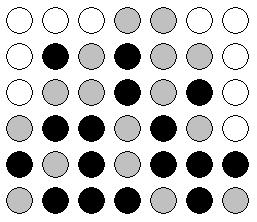
\includegraphics[width=0.8\textwidth]{image/puissance4}
	\end{minipage}
	\begin{minipage}[t][][b]{10cm}
	N.B. : sur ce dessin noir et
	blanc, les jetons rouges apparaissent en noir, les jetons jaunes en
	gris et les cases blanches désignent l'absence de
	jetons. Cet exemple montre une situation du jeu où le joueur «~jaune~»
	est gagnant. En introduisant un jeton dans la
	4\textsuperscript{e} colonne,
	il a réalisé un alignement de 4 jetons en oblique.
	\end{minipage}
	
	On demande d’implémenter une classe Puissance4 qui permette de contrôler
	l’état des différentes phases du jeu. Déterminez les attributs de cette
	classe et décrivez-les brièvement de manière à justifier votre choix.
	Dotez ensuite la classe des méthodes permettant de :

	\begin{itemize}
		\item 
			savoir si la grille est pleine
		\item 
			mettre la grille à jour lorsque le joueur n (1 ou 2) joue dans la
			colonne j (entre 1 et 7). Cette méthode renverra la valeur booléenne
			faux si la colonne en question est déjà pleine
		\item 
			vérifier si le joueur qui vient de jouer dans la colonne j a gagné la
			partie
	\end{itemize}
	
	N.B. : pour la structure qui contiendra le contenu du tableau de jetons,
	on adoptera la convention suivante : 0 pour l’absence de jeton, 1
	représentera un jeton du 1\textsuperscript{er} joueur, et 2 un jeton du
	2\textsuperscript{e} joueur (on peut donc faire abstraction de la
	couleur du jeton dans ce problème).
	
\end{Exercice}

%---------------------------
\begin{Exercice}{Mastermind}
%---------------------------

	Revenons sur le jeu Mastermind déjà vu en DEV1.
	Dans ce jeu, un joueur A doit trouver une combinaison de
	\lda{k} pions de couleur, choisie et tenue secrète
	par un autre joueur B. Cette combinaison peut contenir éventuellement
	des pions de même couleur. À chaque proposition du joueur A, le joueur
	B indique le nombre de pions de la proposition qui sont corrects et
	bien placés et le nombre de pions corrects mais mal placés. 

	\textbf{Exemple}

	Utilisons des lettres pour représenter les couleurs.
	
	\begin{minipage}{5cm}
		\begin{center}
		Combinaison secrète
		
		\begin{tabular}{|*{5}{>{\centering\arraybackslash}m{0.35cm}|}}
			\hline
			R & R & V & B & J \\
			\hline
		\end{tabular}
		\end{center}	
	\end{minipage}
	\
	\begin{minipage}{5cm}
		\begin{center}
		Proposition du joueur
	
		\begin{tabular}{|*{5}{>{\centering\arraybackslash}m{0.35cm}|}}
			\hline
			R & V & B & B & V \\
			\hline
		\end{tabular}
		\end{center}
	\end{minipage}
	
	Il sera indiqué au joueur qu'il a :
	\begin{itemize}
	\item 2 pions bien placés : le R en 1\iere{} position et le
	second B en 4\ieme{} position ;
	\item 1 pion mal placé : un des deux V (ils ne peuvent compter tous les deux).
	\end{itemize}
	
	\medskip
	Supposons une énumération \lda{Couleur}
	(cf. la description d'une énumération en annexe) 
	avec toutes les couleurs possibles de pion.

	\begin{enumerate}[label=\alph*)]
		\item
			Écrire une classe «\lda{~Combinaison~}» pour
			représenter une combinaison de \lda{k} pions. Elle
			possède une méthode pour générer une combinaison aléatoire (que vous ne
			devez pas écrire) et une méthode pour comparer une combinaison à la
			combinaison secrète (que vous devez écrire)
		\item
			Écrire ensuite une classe «\lda{~MasterMind~}» qui
			représente le jeu et permet d’y jouer. La taille de la combinaison et
			le nombre d’essais permis seront des paramètres du constructeur.
	\end{enumerate}
\end{Exercice}






	\appendix
	\chapter{Compléments}

	Nous présentons ici quelques éléments qui pourront
	vous être utiles pour résoudre certains exercices.
	
%===================================================
\section{Énumération}
%===================================================

	Parfois, une variable ne peut prendre 
	qu’un ensemble fixe et fini de valeurs. 
	Par exemple une variable représentant une saison 
	ne peut prendre que quatre valeurs (HIVER, PRINTEMPS, ÉTÉ, AUTOMNE). 
	On va l’indiquer grâce à l’énumération 
	qui introduit un \textbf{nouveau type} de donnée.

	\begin{LDA}
		\Stmt \K{enum} Saison \{ HIVER, PRINTEMPS, ÉTÉ, AUTOMNE \}
	\end{LDA}

	Il y a deux avantages à cela~:~
	une indication claire des possibilités de la variable lors de la déclaration 
	et une lisibilité du code grâce à l’utilisation des valeurs explicites.

	Par exemple, 

	\begin{LDA}
		\LComment Lit une saison et affiche sa particularité
		\Algo{particularitéSaisonnière}{}{}
			\Decl{uneSaison}{Saison}
			\Read uneSaison
			\RComment on lira la valeur HIVER ou PRINTEMPS ou ÉTÉ ou AUTOMNE
			\If{uneSaison = HIVER}
				\Write "il neige"
			\ElsIf{uneSaison = PRINTEMPS}
				\Write "les fleurs poussent"
			\ElsIf{uneSaison = ÉTÉ}
				\Write "le soleil brille"
			\Else
				\Write "les feuilles tombent"
			\EndIf
		\EndAlgo
	\end{LDA}


	\begin{Exercice}{Autres situations}
	
		Pouvez-vous identifier d’autres données qui pourraient
		avantageusement s’exprimer avec une énumération~?
	
	\end{Exercice}

	\subsection{Quid des langages de programmation~?}
	%-------------------------------------------------
	
		Certains langages (comme Java) proposent un type énuméré complet.
		D’autres (comme C et C++) proposent un type énuméré incomplet 
		mais qui permet néanmoins une écriture comme celle ci-dessus.
		Cobol propose des «~noms conditions~» qui représentent
		l’ensemble des valeurs possibles d’une variable. 
		D’autres langages, enfin, ne proposent rien. 
		Pour ces langages, le truc est de définir des constantes entières 
		qui vont permettre une écriture proche de celle ci-dessus 
		(mais sans une déclaration explicite).

	\subsection{Lien avec les entiers}
	%-------------------------------------
	
		Dans l’exemple ci-dessus, on lit une Saison mais souvent,
		si on travaille avec les Mois par exemple,
		on disposera plutôt d’un entier. 
		Il faut pouvoir convertir les valeurs. 
		Chaque langage de programmation propose sa propre technique; 
		nous allons adopter la syntaxe suivante~:

		\begin{LDA}
			\Stmt Saison(3) 
				\RComment donne l’énumération de la saison numéro 3 (on commence à 1);
				\Stmt\RComment donne ÉTÉ dans notre exemple.
			\Stmt position(uneSaison)
				\RComment donne l’entier associé à une saison;
				\Stmt\RComment si on a lu HIVER comme valeur pour uneSaison, donne la valeur 1.
		\end{LDA}
		
	
	%===================================================
	\section{Gestion des erreurs}
	%===================================================

		Lorsqu'un algorithme se trouve dans un état incorrect,
		particulièrement lorsqu'un paramètre est invalide,
		on peut l'indiquer via la primitive \lda{\K{erreur}}.
	
		Par exemple :	
		\begin{LDA}
			\Algo{racineCarrée}{\Par{nb}{entier}}{}
				\If{nb<0}
					\Error{"Le nombre doit être positif"}
				\EndIf
				\Stmt suite de l'algorithme...
			\EndAlgo
		\end{LDA}
			
		Pratiquement, cette primitive stoppe l'algorithme
		sans aucune possibilité de récupération.
		Dans un langage comme \bsc{Java} vous utiliserez
		le mécanisme des exceptions qui est plus souple. 
	\chapter{Aide mémoire}

	Cet aide-mémoire peut vous accompagner lors d'une
	interrogation ou d'un examen. 
	Il vous est permis d’utiliser ces méthodes sans les développer.
	Par contre, si vous sentez le besoin d’utiliser 
	une méthode qui n'apparait pas ici, 
	il faudra en écrire explicitement le contenu.

%===================================================
\section{Manipuler le hasard}
%===================================================

	\begin{algo}
	\MethodSign{hasard}{}{réel}
		\RComment{Donne un nombre réel entre 0 inclus et 1 exclu.}
	\MethodSign{hasard}{\Par{n}{entier}}{réel}
		\RComment{Donne un nombre entre entre 0 inclus et \lda{n} exclu.}
	\MethodSign{hasard}{\Par{min}{entier}, \Par{max}{entier}}{entier}
		\RComment{Donne un entier entre \lda{min} et \lda{max} inclus.}
	\end{algo}
		
%===================================================
\section{La liste}
%===================================================
	
\begin{algo}
	\Comment{T est un type quelconque}\;
	\Class{\List{T}}{
		\Public{
			\ConstrSign{\List{T}}{}
			\RComment{construit une liste vide}
			\MethodSign{get}{pos : integer}{T}
			\RComment{donne un élément en position pos}
			\MethodSign{set}{pos : integer, valeur : T}{}
			\RComment{modifie un élément en position pos}
			\MethodSign{size}{}{integer}
			\RComment{donne le nombre actuel d’éléments}
			\MethodSign{isEmpty}{}{boolean}
			\RComment{la liste est-elle vide ?}
			\MethodSign{add}{value : T}{}
			\RComment{ajoute un élément en fin de liste}
			\MethodSign{add}{pos : integer, value : T}{}
			\RComment{insère un élément en position pos}
			\MethodSign{removePos}{pos : integer}{}
			\RComment{supprime l'élément en position pos}
			\MethodSign{remove}{value : T}{boolean}
			\RComment{supprime l'élément de valeur donnée}
			\MethodSign{clear}{}{}
			\RComment{vide la liste}
			\MethodSign{contains}{value : T}{boolean}
			\RComment{indique si un élément est présent}
			\MethodSign{indexOf}{value : T}{integer}
			\RComment{donne la position d'un élément}
		}
	}
\end{algo}


\end{document}
